% (c)~2014 Dimitrios Vrettos - d.vrettos@gmail.com
% (c)~2014 Claudio Carboncini - claudio.carboncini@gmail.com
\chapter{Disequazioni di secondo grado}

\section{Risoluzione delle disequazioni di secondo grado}

Una disequazione di secondo grado si presenta in una delle seguenti forme:
\[ax^2+bx+c>0;\quad ax^2+bx+c\ge 0;\quad ax^2+bx+c<0;\quad ax^2+bx+c\le 0.\]

Per risolverla supponiamo che il coefficiente di $x^2$, cioè il coefficiente $a$, sia \textit{positivo}. Se così non fosse, basterebbe cambiare segno a tutti i termini e quindi il verso della disequazione; per esempio, per risolvere la disequazione $-2x^2+3x-1>0$ si può risolvere la disequazione $2x^2-3x+1<0$.

Per risolvere una disequazione di secondo grado si risolve l'equazione associata, cioè si sostituisce il segno della disequazione con l'uguale. Si passa cioè dalla disequazione $ax^2+bx+c>0$ all'equazione $ax^2+bx+c=0$.

Possono presentarsi tre casi.

\subsection{Equazione spuria}
Sono equazioni senza il termine noto: $ax^2+bx=0$.

Questa equazione ammette sempre due radici reali e distinte, di cui una è sempre $0$. Ricordiamo che l'equazione si risolve mettendo $x$ a fattore comune $x(ax+b)=0$ e applicando la legge di annullamento del prodotto, da cui ricaviamo $x=0\ \vee \ ax+b=0\rightarrow x=-\frac b a$. Chiamiamo le due radici $x_1$ e $x_2$. Analogamente a quanto fatto nelle disequazioni di primo grado, poniamo separatamente ogni fattore maggiore di $0$ e confrontiamo i segni dei singoli fattori, come nel seguente grafico.
\begin{center}
% (c) 2013 Claudio Carboncini - claudio.carboncini@gmail.com
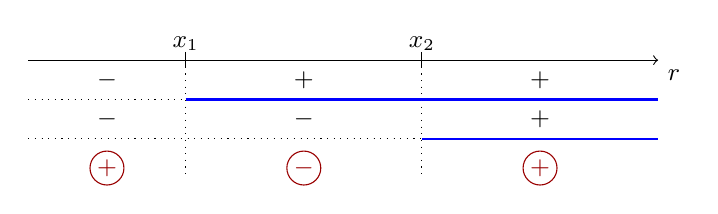
\begin{tikzpicture}[font=\small,x=10mm, y=10mm]

\draw[->] (0,0) -- (8,0) node [below right] () {$r$};

\foreach \x in {2,5}{
\draw(\x,3pt)--(\x,-3pt);
\begin{scope}[dotted]
\draw (\x,0) -- (\x,-1.5);
\draw (0,-1) -- (5,-1);
\draw (0,-.5) -- (2,-.5);
\end{scope}}

\node[above]  at (2,0) {$x_1$};
\node[above]  at (5,0) {$x_2$};

\begin{scope}[blue,thick]
\draw (5,-1) -- (8,-1);
\draw (2,-.5) -- (8,-.5);
\end{scope}

\foreach \z in {3.5,6.5}{
\node  at (\z,-.25) {$+$};
}
\foreach \zi in {1, 3.5}{
\node  at (\zi,-.75) {$-$};
}

\node  at (1,-.25) {$-$};
\node  at (6.5,-.75) {$+$};

\begin{scope}[red!60!black]
\foreach \zii in {1, 6.5}{
\node[circle,inner sep=1pt,draw]  at (\zii,-1.37){$+$};
}
\node[circle,inner sep=1pt,draw]  at (3.5,-1.37) {$-$};
\end{scope}
\end{tikzpicture}

\end{center}
Dal grafico si evince che le soluzioni saranno:
\begin{itemize}
\item $x<x_1\vee x>x_2$ soluzioni esterne se la disequazione è $ax^2+bx>0$, analogamente $x\le x_1\vee x\ge x_2$ se la disequazione è $ax^2+bx\ge 0$.
\item $x_1<x<x_2$ soluzioni interne se la disequazione è $ax^2+bx<0$, analogamente $x_1\le x\le x_2$ se la disequazione è $ax^2+bx\le 0$.
\end{itemize}
\pagebreak
\begin{exrig}
\begin{esempio}
Risolvere le seguenti disequazioni spurie.
\begin{itemize}
\item $3x^2-2x>0$.

Mettiamo $x$ a fattore comune $x(3x-2)>0$.

Poiché il verso della disequazione è ``$>0$'' la disequazione è verificata per valori esterni alle soluzioni dell'equazione, cioè:  $x<0\vee x>\frac 2 3$;
\item $5x^2+x\le 0$.

Mettiamo $x$ a fattore comune $x(5x+1)\le 0$.

Poiché il verso della disequazione è ``$\le 0$'' la disequazione è verificata per valori interni alle soluzioni dell'equazione, cioè: $-\frac 1 5\le x\le 0$;
\item $x-3x^2>0$ cambiamo di segno $3x^2-x<0$ da cui $x(3x-1)<0$. Soluzioni: $0<x<\frac 1 3$.
\end{itemize}
\end{esempio}
\end{exrig}

\subsection{Equazione pura}
Sono equazioni senza il termine con la $ x $: $ax^2+c=0$.

Possono esserci due situazioni:
\begin{itemize}
\item $c<0$: in questo caso l'equazione ammette due radici reali opposte: $x_{1\text{,}2}=\pm \sqrt{-\frac c a}$: si torna al caso precedente e si ha $x<x_1\vee x>x_2$ (cioè per valori esterni) se la disequazione è $ax^2+c>0$ oppure $x_1<x<x_2$ (cioè per valori interni) se la disequazione è $ax^2+c<0$;
\item $c>0$: l'equazione non ammette soluzioni reali; il binomio $ax^2+c$ è la somma di un quadrato con un numero positivo, pertanto è sempre positivo. Di conseguenza, la disequazione $ax^2+c>0$ avrà soluzioni per ogni $x$ reale, mentre $ax^2+c<0$ non avrà nessuna soluzione reale.
\end{itemize}

\begin{exrig}
\begin{esempio}
Risolvere le seguenti disequazioni pure.
\begin{itemize}
\item $x^2-4\ge 0$ soluzioni $x\le -2\vee x\ge 2$;
\item $2x^2-18\le 0$ soluzioni $-3\le x\le 3$;
\item $x^2+4>0$ soluzioni $\forall x\in \insR$;
\item $x^2+9\le 0$ soluzioni nessun valore reale $\IS=\emptyset$;
\item $1-x^2<0$ cambiamo di segno $x^2-1>0$ soluzioni $x<-1\vee x>1$.
\end{itemize}
\end{esempio}
\end{exrig}

\pagebreak

\subsection{Equazione completa}
Sono equazioni con tutti i coefficienti diversi da zero: $ax^2+bx+c=0$.

Si calcola il valore del discriminante $\Delta =b^2-4{ac}$ e a secondo del suo segno possono presentarsi tre casi:

\paragraph{Primo caso: $\Delta >0$}
L'equazione ammette due radici reali e distinte $x_1$ e $x_2$ e il trinomio si scompone in $a(x-x_1)(x-x_2)$. Poiché abbiamo supposto $a$ positivo, il segno del trinomio è dato, per il teorema dui Cartesio, dal seguente schema (ponendo $x_1<x_2$):
\begin{center}
% (c) 2013 Claudio Carboncini - claudio.carboncini@gmail.com
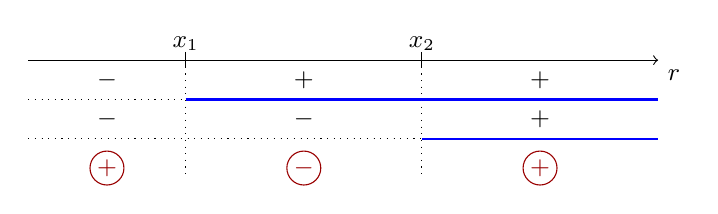
\begin{tikzpicture}[font=\small,x=10mm, y=10mm]

\draw[->] (0,0) -- (8,0) node [below right] () {$r$};

\foreach \x in {2,5}{
\draw(\x,3pt)--(\x,-3pt);
\begin{scope}[dotted]
\draw (\x,0) -- (\x,-1.5);
\draw (0,-1) -- (5,-1);
\draw (0,-.5) -- (2,-.5);
\end{scope}}

\node[above]  at (2,0) {$x_1$};
\node[above]  at (5,0) {$x_2$};

\begin{scope}[blue,thick]
\draw (5,-1) -- (8,-1);
\draw (2,-.5) -- (8,-.5);
\end{scope}

\foreach \z in {3.5,6.5}{
\node  at (\z,-.25) {$+$};
}
\foreach \zi in {1, 3.5}{
\node  at (\zi,-.75) {$-$};
}

\node  at (1,-.25) {$-$};
\node  at (6.5,-.75) {$+$};

\begin{scope}[red!60!black]
\foreach \zii in {1, 6.5}{
\node[circle,inner sep=1pt,draw]  at (\zii,-1.37){$+$};
}
\node[circle,inner sep=1pt,draw]  at (3.5,-1.37) {$-$};
\end{scope}
\end{tikzpicture}

\end{center}
Pertanto la disequazione ${ax}^2+{bx}+c\ge 0$ è verificata per valori esterni alle soluzioni, cioè $x\le x_1\vee x\ge x_2$; mentre la disequazione ${ax}^2+{bx}+c\le 0$ è verificata per valori interni alle soluzioni, cioè $x_1\le x\le x_2$.

\begin{exrig}
\begin{esempio}
Risolvere le seguenti disequazioni complete con $\Delta>0$.
\begin{itemize}
\item $x^2-3x-4>0$. Calcolo il valore del discriminante $\Delta =9+16=25$ e le soluzioni dell'equazione associata $x_1=-1\,\vee\,x_2=4$. Le soluzioni della disequazione sono: $x<-1\,\vee\,x>4$;
\item $x^2-3x-4<0$. In questo caso le soluzioni della disequazione sono $-1<x<4$.
\end{itemize}
\end{esempio}
\end{exrig}

\paragraph{Secondo caso: $\Delta =0$} In questo caso le radici dell'equazione associata sono coincidenti $x_1=x_2$, pertanto il trinomio si scompone in $a(x-x_1)^2$. Poiché $a$ è positivo e il quadrato è positivo o al più nullo, si possono verificare quattro casi:

\begin{itemize*}
\item $a(x-x_1)^2>0\:$ è verificata $\forall x\in \insR- \{x_1\}$;
\item $a(x-x_1)^2\ge 0\:$ è verificata $\forall x\in \insR$;
\item $a(x-x_1)^2<0\:$ non è mai verificata;
\item $a(x-x_1)^2\le 0\:$ è verificata solo per $x=x_1$.
\end{itemize*}

\begin{exrig}
\begin{esempio}
Risolvere le seguenti disequazioni complete con $\Delta=0$.
\begin{itemize}
\item $x^2-2x+1>0$. Si ha $(x-1)^2>0$ che è verificata $\forall x\in \insR - \{1\}$;
\item $4x^2-4x+1\ge 0$. Si ha $(2x-1)^2\ge 0$ che è verificata $\forall x\in \insR$;
\item $x^2+2x+1<0$. Si ha $(x+1)^2<0$ che non è mai verificata;
\item $4x^2+4x+1\le 0$. Si ha $(2x+1)^2\le 0$ che è verificata solo per $x=-\frac 1 2$.
\end{itemize}
\end{esempio}
\end{exrig}

\paragraph{Terzo caso: $\Delta <0$} Studiamo il segno che assume il trinomio in questo caso. Dobbiamo eseguire i seguenti passaggi:

\begin{itemize*}
\item mettiamo il coefficiente $a$ a fattore comune, aggiungendo e togliendo $\frac{b^2} {4a^2}$ ottenendo 
\[{ax}^2+{bx}+c=a\left(x^2+\frac b ax+\frac{b^2} {4a^2}-\frac{b^2} {4a^2}+\frac c a\right);\]
\item osserviamo che i primi tre termini costituiscono lo sviluppo del quadrato di un binomio, e riduciamo gli ultimi due allo stesso denominatore ottenendo 
\[a\left[\left(x+\frac b {2a}\right)^2-\frac{b^2-4{ac}} {4a^2}\right];\]
\item studiamo ora il segno di questa espressione: $a$ è positivo, nella parentesi quadra si ha una somma in cui $\left(x+\frac b {2a}\right)^2$ essendo un quadrato è sempre positivo, come $-\frac{b^2-4{ac}} {4a^2}=-\frac{\Delta } {4a^2}$ sempre positivo perché $\Delta <0$. Possiamo allora concludere che il trinomio è sempre positivo.
\end{itemize*}
Si hanno allora le seguenti possibilità con $a>0$:

\begin{itemize*}
\item ${ax}^2+{bx}+c>0$ è verificata $\forall x\in \insR$;
\item ${ax}^2+{bx}+c\ge 0$ è verificata $\forall x\in \insR$ (anche se non può mai essere uguale a zero);
\item ${ax}^2+{bx}+c<0$ non è mai verificata;
\item ${ax}^2+{bx}+c\le 0$ non è mai verificata.
\end{itemize*}

\begin{exrig}
\begin{esempio}
Risolvere le seguenti disequazioni complete con $\Delta<0$.
\begin{itemize*}
\item $2x^2-3x+4>0$. Si ha $\Delta =9-32=-23<0$, verificata $\forall x\in \insR$;
\item $x^2-x+1<0$. Si ha $\Delta =1-4=-3<0$, mai verificata per alcun valore reale di $x$.
\end{itemize*}
\end{esempio}
\end{exrig}

I seguenti esempi analizzano la risoluzione di disequazioni di secondo grado con $\Delta \ge 0$.
\begin{exrig}
\begin{esempio}
Determinare l'insieme soluzione della disequazione $-3x^2+2x>0$.

Cambiamo segno per avere il primo coefficiente positivo; la disequazione si trasforma in $3x^2-2x<0$; l'equazione associata è spuria $3x^2-2x=0$ con le radici $x_1=0\vee x_2=\frac 2 3$. Pertanto la disequazione assegnata ha $\IS=\left\{x\in \insR \mid 0<x<\frac 2 3\right\}$.
\end{esempio}

\begin{esempio}
Determinare l'insieme soluzione della disequazione $2x^2-5\le 0$.

L'equazione associata $2x^2-5=0$ è pura con soluzioni reali $x=\pm \sqrt{\frac 5 2}$. Razionalizzando otteniamo: $x_1=-\frac{\sqrt{10}} 2\vee x_2=+\frac{\sqrt{10}} 2$ e quindi $\IS=\left\{x\in \insR \mid -\frac{\sqrt{10}} 2\le x\le +\frac{\sqrt{10}} 2\right\}$.
\end{esempio}

\begin{esempio}
Determinare l'insieme soluzione della disequazione $2x^2+3x-1>0$.

L'equazione associata è completa $2x^2+3x-1=0$; $\Delta =9+8=17>0$ è positivo, dunque le soluzioni sono $x_1=\frac{-3-\sqrt{17}} 4\vee x_2=\frac{-3+\sqrt{17}} 4$. Ci troviamo nel primo caso, quindi l'insieme soluzione della disequazione è~$\IS=\left\{x\in \insR \mid x<\frac{-3-\sqrt{17}} 4\vee x>\frac{-3+\sqrt{17}} 4\right\}$.
%
%Osserviamo che contemporaneamente sappiamo anche risolvere le altre disequazioni: $2x^2+3x-1<0$,~~$2x^2+3x-1\ge 0$~~e~~$2x^2+3x-1\le 0$.
\end{esempio}
\end{exrig}
\conclusione Una disequazione di secondo grado si presenta sempre in una delle seguenti forme: ${ax}^2+{bx}+c>0$, ${ax}^2+{bx}+c\ge 0$, ${ax}^2+{bx}+c<0$, ${ax}^2+{bx}+c\le 0$; possiamo sempre supporre positivo il primo coefficiente e, anche se incompleta, per l'equazione associata possiamo sempre pensare ai tre casi generati dal segno del discriminante $\Delta =b^2-4{ac}$.

Pertanto l'insieme soluzione $\IS$ segue lo schema riportato nella seguente tabella:
\begin{center}
\begin{threeparttable}
\begin{tabular}{lcccc}
\toprule
Delta & $ax^2+bx+c>0$& $ax^2+bx+c\ge0$& $ax^2+bx+c<0$ & $ax^2+bx+c\le0$\\
\midrule
 $\Delta >0^{*}$& $ x<x_1\vee x>x_2 $ & $ x\le x_1\vee x\ge x_2 $& $ x_1<x<x_2 $&$ x_1\le x\le x_2 $\\
$\Delta =0^{**}$& $\forall x\in \insR-\{x_1\} $ & $ \forall x\in \insR $& $ \IS=\emptyset $&$ x=x_1=x_2 $\\
$\Delta <0^{***}$&$ \forall x\in \insR $ & $ \forall x\in \insR $& $ \IS=\emptyset $&$ \IS=\emptyset $\\
\bottomrule
\end{tabular}
\begin{tablenotes}
\item [*] l'equazione associata ha 2 soluzioni reali distinte: $x=x_1\vee x=x_2$.
\item [**] l'equazione associata ha 2 soluzioni reali coincidenti: $x=x_1=x_2$.
\item [***] l'equazione associata non ha soluzioni reali.
\end{tablenotes}
\end{threeparttable}
\end{center}

\vspazio\ovalbox{\risolvii \ref{ese:4.1}, \ref{ese:4.2}, \ref{ese:4.3}, \ref{ese:4.4}, \ref{ese:4.5}}

\section{Risoluzione grafica di una disequazione di secondo grado}

Ricordiamo che un polinomio in una sola variabile, solitamente indicata con $x$, è di secondo grado se $2$ è il massimo esponente della variabile. Per \emph{trinomio di secondo grado} intendiamo un polinomio di secondo grado: $ax^2+bx+c$ con $a\in \insR_{0}$ e $b$, $c\in \insR$. Chiamiamo \emph{zeri del trinomio} i numeri reali soluzione dell'equazione associata $ax^2+bx+c=0$.

\begin{figure}[b]
 \begin{minipage}[t]{.45\textwidth}
\centering
 % (c) 2013 Claudio Carboncini - claudio.carboncini@gmail.com
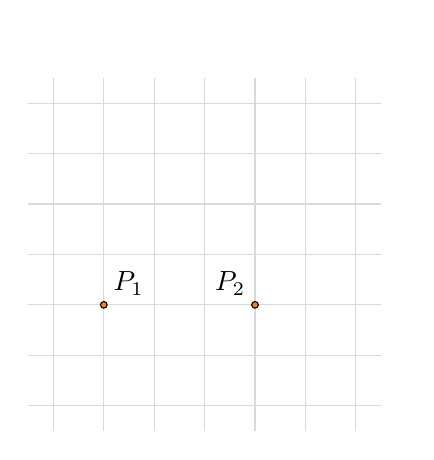
\begin{tikzpicture}[x=8mm, y=8mm,scale=.8 ]
\draw[step=0.8cm,color=gray!30] (-3.5,-2.5) grid (3.5,4.5);
  \tkzInit[xmin=-3,xmax=3,ymin=-2.5,ymax=3.5]
  \clip (-3.5,-2.5) rectangle (4,5.5);
  \begin{scope}[font=\small]
    \tkzAxeY[orig = false, label options={left = 1pt}]
    \tkzAxeX[orig = true, label options={below = 1pt}]
  \end{scope}
  \tkzFct[domain=-3:2,thick,color=Maroon]{x*x+x-2};
  \draw[fill=orange] (-2,0)circle (1.5pt);
  \node[above right] at (-2,0) {$P_1$};
  \draw[fill=orange] (1,0)circle (1.5pt);
  \node[above left] at (1,0) {$P_2$};

\end{tikzpicture}

\caption{La funzione~$y=x^{2}+x-2$.}\label{fig:4.1}
 \end{minipage}\hfil
 \begin{minipage}[t]{.45\textwidth}
\centering
 % (c) 2013 Claudio Carboncini - claudio.carboncini@gmail.com
% (c) 2014 Dimitrios Vrettos - d.vrettos@gmail.com
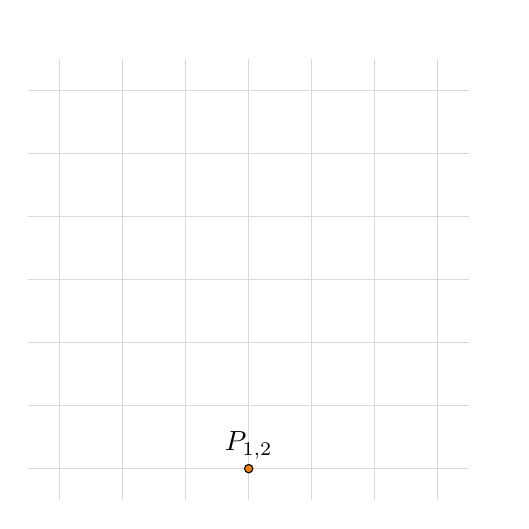
\begin{tikzpicture}[x=8mm, y=8mm]

\draw[step=0.8cm,color=gray!30] (-1.5,-.5) grid (5.5,6.5);
  \tkzInit[xmin=-1,xmax=5,ymin=0,ymax=5.5]
  \clip (-1.5,-.5) rectangle (6,7);
  \begin{scope}[font=\small]
    \tkzAxeY[orig = false, label options={left = 1pt}]
    \tkzAxeX[orig = true, label options={below = 1pt}]
  \end{scope}
  \tkzFct[domain=-1:5,thick,color=Maroon]{x*x-4*x+4};
  \draw[fill=orange] (2,0)circle (1.5pt);
  \node[above] at (2,0) {$P_{1\text{,}2}$};

\end{tikzpicture}

\caption{La funzione~$y=x^{2}-4x+4$.}\label{fig:4.2}
 \end{minipage}
\end{figure}

\begin{definizione}
Una funzione $f$ che associa ad ogni numero $x\in \insR$ il valore $y=ax^2+bx+c$ con $a\in \insR_{0}$ e $b$, $c\in \insR$ si chiama \emph{funzione polinomiale di secondo grado}.
\end{definizione}

Nel riferimento cartesiano ortogonale, il grafico della funzione $f$ è costituito da tutti e soli i punti le cui coordinate soddisfano l'equazione $y=ax^2+bx+c$; se $x_1$ e $x_2$ sono gli zeri reali del trinomio $ax^2+bx+c$ significa che attribuendo tali valori alla variabile $x$ si ha $y=0$; essi sono dunque gli \emph{zeri della funzione}, ossia le ascisse dei punti del grafico appartenenti all'asse $x$.
\pagebreak
\begin{exrig}
\begin{esempio}
\label{ex:4.9}
Determinate gli zeri del trinomio $x^2+x-2$.

Risolviamo l'equazione $x^2+x-2=0$ che avendo il discriminante positivo ammette due soluzioni reali distinte $x_1=-2\vee x_2=1$. I due numeri $1$ e $-2$ sono gli zeri della funzione $y=x^2+x-2$ (figura~\ref{fig:4.1} a pagina~\pageref{fig:4.1}). Nel riferimento cartesiano ortogonale i punti $P_1(-2;0)$ e $P_2(1;0)$ sono i punti del grafico della funzione appartenenti all'asse $x$.
\end{esempio}

\begin{esempio}
\label{ex:4.10}
Determinate gli zeri del trinomio $x^2-4x+4$.

Risolviamo l'equazione $x^2-4x+4=0$ che avendo il discriminante nullo ammette due soluzioni reali coincidenti $x_1=x_2=2$, gli zeri del trinomio sono coincidenti nel numero $2$ e il grafico della funzione $y=x^2-4x+4$  (figura~\ref{fig:4.2} a pagina~\pageref{fig:4.2}) ha quindi due punti coincidenti appartenenti all'asse~$x$: $P_1\equiv P_2(2;0)$.
\end{esempio}
%\newpage
%\pagebreak

\begin{esempio}
\label{ex:4.11}
Determinate gli zeri del trinomio $x^2-2x+5$.

Risolviamo l'equazione $x^2-2x+5=0$ che avendo il discriminante negativo non ammette soluzioni reali; il trinomio non ha zeri reali e il grafico della funzione $y=x^2-2x+5$ (figura~\ref{fig:4.3} a pagina~\pageref{fig:4.3}) non ha punti appartenenti all'asse~$x$.
\end{esempio}
\end{exrig}

Questi esempi ci hanno permesso di chiarire il collegamento tra il concetto algebrico ``zeri di un polinomio'' e il concetto geometrico di ``punti sull'asse delle ascisse'' del grafico della funzione polinomiale di secondo grado. Pertanto studiare il \emph{segno di un trinomio di secondo grado} equivale a determinare quali sono le \emph{ascisse dei punti} della funzione $y=ax^2+bx+c$ (con $a\in \insR_{0}$ e $b$, $c\in \insR$) che hanno \emph{ordinata positiva} oppure \emph{ordinata negativa}.

Ricordiamo che nel riferimento cartesiano ortogonale i punti ad ordinata positiva si trovano nel I e nel II quadrante (cioè al di sopra dell'asse~$x$), i punti ad ordinata negativa si trovano nel III e nel IV quadrante (cioè al di sotto dell'asse~$x$) e i punti ad ordinata nulla si trovano sull'asse~$x$.

Per studiare il segno del trinomio, dobbiamo quindi tracciare, nel riferimento cartesiano, il grafico della funzione $y=ax^2+bx+c$ (con $a\in \insR_{0}$ e $b$, $c\in \insR$).

\begin{figure}[b]
 \begin{minipage}[t]{.45\textwidth}
\centering
 % (c) 2013 Claudio Carboncini - claudio.carboncini@gmail.com
% (c) 2014 Dimitrios Vrettos - d.vrettos@gmail.com
\begin{tikzpicture}[x=8mm, y=8mm]

\draw[step=0.8cm,color=gray!30] (-1.5,-.5) grid (4.5,6.5);
  \tkzInit[xmin=-1,xmax=4,ymin=0,ymax=5.5]
  \clip (-1.5,-.5) rectangle (6,6.5);
  \begin{scope}[font=\small]
    \tkzAxeY[orig = false, label options={left = 1pt}]
    \tkzAxeX[orig = true, label options={below = 1pt}]
  \end{scope}
  \tkzFct[domain=-1:3,thick,color=Maroon]{x*x-2*x+2};

\end{tikzpicture}

\caption{La funzione~$y=x^{2}-2x+5$.}\label{fig:4.3}
 \end{minipage}\hfil
 \begin{minipage}[t]{.45\textwidth}
\centering
 % (c) 2013 Claudio Carboncini - claudio.carboncini@gmail.com
% (c) 2014 Dimitrios Vrettos - d.vrettos@gmail.com

\begin{tikzpicture}[x=8mm, y=8mm]
\draw[step=0.8cm,color=gray!30] (-3.5,-.5) grid (3.5,6.5);
  \tkzInit[xmin=-3,xmax=3,ymin=-1,ymax=5]
  \clip (-3.5,-.5) rectangle (4,6.5);
  \begin{scope}[font=\small]
    \tkzAxeY[orig = false, label options={left = 1pt}]
    \tkzAxeX[orig = true, label options={below = 1pt}]
  \end{scope}
  \tkzFct[domain=-2:2,thick,color=Maroon]{2*x*x}
\end{tikzpicture}

\caption{La funzione $y=2x^2$.}\label{fig:4.4}
 \end{minipage}
\end{figure}

\subsection{Rappresentazione di una funzione polinomiale di secondo grado nel piano cartesiano}

Consideriamo la funzione $y=2x^2$ (figura~\ref{fig:4.4} a pagina~\pageref{fig:4.4}) di proporzionalità quadratica definita in tutto $\insR$; sappiamo che il suo grafico è una parabola che volge la concavità verso l'alto essendo il coefficiente della variabile indipendente positivo e che il punto $O(0;0)$ è il suo vertice. Per tracciarne il grafico compiliamo una tabella e riportiamo i punti nel riferimento cartesiano.

\begin{center}
\begin{tabular} {*{8}{c}}
\toprule
$x$      & $\np{-1,5}$ & $-1$ & $\np{-0,5}$ & $0$ & $\np{0,5}$ & $1$ & $\np{1,5}$\\
$y=2x^2$ & $ \np{4,5}$ &  $2$ &  $\np{0,5}$ & $0$ & $\np{0,5}$ & $2$ & $\np{4,5}$\\
\bottomrule
\end{tabular}
\end{center}

Applichiamo a tutti i punti della tabella la traslazione di vettore $\vec u(1;1)$. Sappiamo che la traslazione modifica le coordinate dei punti secondo il sistema ${T}(1;1) \left\{\begin{array}{l}{x'=x+1}\\{y'=y+1}\end{array}\right.$ quindi possiamo compilare la tabella dei punti corrispondenti di $x$ e $y$ secondo $T(1;1)$ e infine tracciare il grafico della parabola immagine di $y=2x^2$.

\begin{center}
\begin{tabular} {*{8}{c}}
\toprule
$x'$ & $\np{-0,5}$ & $0$ & $\np{0,5}$ & $1$ & $\np{1,5}$ & $2$ & $\np{2,5}$\\
$y'$ & $\np{5,5}$  & $3$ & $\np{1,5}$ & $1$ & $\np{1,5}$ & $3$ & $\np{5,5}$\\
\bottomrule
\end{tabular}
\end{center}

\begin{center}
 % (c) 2013 Claudio Carboncini - claudio.carboncini@gmail.com
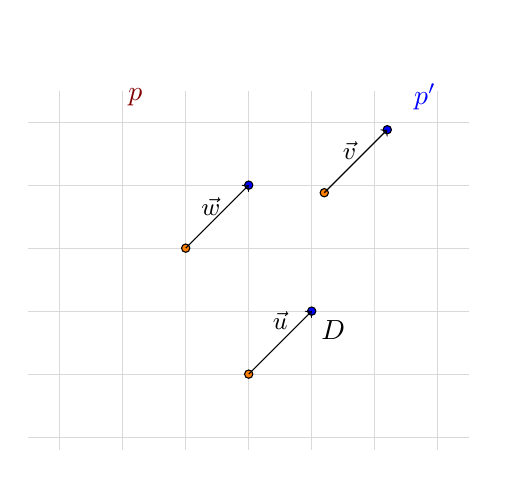
\begin{tikzpicture}[x=8mm, y=8mm]
\draw[step=0.8cm,color=gray!30] (-3.5,-1.2) grid (3.5,4.5);
  \tkzInit[xmin=-3,xmax=3,ymin=-1,ymax=4.5]
  \clip (-3.5,-1.5) rectangle (4,5.5);
  \begin{scope}[font=\small]
    \tkzAxeY[orig = false, label options={left = 1pt}]
    \tkzAxeX[orig = true, label options={below = 1pt}]
    \node [label={[name=label node]$\vec{u}$}] at (.5,.4) {};
    \node [label={[name=label node]$\vec{w}$}] at (-.6,2.2) {};
    \node [label={[name=label node]$\vec{v}$}] at (1.6,3.1) {};
  \end{scope}
  \tkzFct[domain=-2:2,thick,color=Maroon]{2*x*x}
  \tkzFct[domain=-2:4,thick,color=blue]{2*x*x-4*x+3};
  %il vettore u
  \draw[fill=orange] (0,0)circle (1.5pt);
  \draw[fill=blue] (1,1)circle (1.5pt);
  \draw[->] (0,0) --(1,1);
  %il vettore w
  \draw[fill=orange] (-1,2)circle (1.5pt);
  \draw[fill=blue] (0,3)circle (1.5pt);
  \draw[->] (-1,2) --(0,3);
  %il vettore v
  \draw[fill=orange] (1.2,2.88)circle (1.5pt);
  \draw[fill=blue] (2.2,3.88)circle (1.5pt);
  \draw[->] (1.2,2.88) --(2.2,3.88);
  \node [color=Maroon] at (-1.8,4.4) {$p$};
  \node [color=blue] at (2.8,4.4) {$p'$};
  \node [below right] at (1,1) {$D$};
\end{tikzpicture}

\end{center}
Dal grafico possiamo leggere le seguenti informazioni:
\begin{itemize}
\item l'immagine della parabola iniziale $p$, è ancora una parabola $p'$ essendo la traslazione una isometria;
\item la parabola $p'$ volge la concavità verso l'alto, come la parabola iniziale $p$;
\item il vertice $O(0;0)$ della parabola $p$ ha come immagine il vertice $D(1;1)$ della parabola $p'$, coincidente con l'estremo libero del vettore $\vec u(1;1)$ che definisce la traslazione;
\item il vettore che individua la traslazione è indicato nella figura con $\vec u$; i vettori $\vec v$ e $\vec w$ rappresentano lo stesso vettore applicato a tre punti presi a caso sulla parabola iniziale.
\end{itemize}
La parabola immagine di $y=2x^2$ è rappresentata da una funzione polinomiale di secondo grado che si ottiene ricavando dal sistema ${T}(1;1)$ le coordinate $\left\{\begin{array}{l}{x=x'-1}\\{y=y'-1}\end{array}\right.$ che, sostituite nell'equazione di $p$ $(y'-1)=2\cdot (x'-1)^2$, permettono di ottenere l'equazione di $p'$: $y=2x^2-4x+3$.

\paragraph{Generalizziamo}
Data la parabola di equazione $y=ax^2$ e la traslazione \[{T}(v_x;v_y)\left\{\begin{array}{l}{x'=x+v_x}\\{y'=y+v_y}\end{array}\right.\text{,}\] per ottenere l'equazione della curva immagine ricaviamo $\left\{\begin{array}{l}{x=x'-v_x}\\{y=y'-v_y}\end{array}\right.$ da sostituire nell'equazione $y={ax}^2$. Da $(y'-v_y)=a\cdot (x'-v_x)^2$ svolgendo i calcoli si ottiene \[y'=a(x')^2-(2av_x)x'+a(v_x)^2+v_y.\] Se poniamo $-2{av}_x=b$ e $a(v_x)^2+v_y=c$ l'equazione della parabola $p'$ immagine di quella data è $y={ax}^2+{bx}+c$, espressa attraverso un polinomio di secondo grado.
\paragraph{Viceversa}
Assegnata la funzione polinomiale di secondo grado $y={ax}^2+{bx}+c$ con $a\neq 0$, sappiamo che il grafico di tale curva è una parabola. In particolare:
\begin{itemize}
\item il coefficiente $a$ indica la concavità: verso l'alto se $a>0$, verso il basso se $a<0$;
\item il coefficiente $c$ indica l'intersezione della parabola con l'asse delle~$y$;
\item dalle formule $-2av_x=b$ e $a(v_x)^2+v_y=c$ ricaviamo le coordinate del suo vertice $v_x=-\frac b{2a}$~~e~~$v_y=c-a\left(-\frac b{2a}\right)^2=\frac{4ac-b^2}{4a}=-\frac{\Delta }{4a}$;
\item risolvendo l'equazione ${ax}^2+{bx}+c=0$ determiniamo gli eventuali punti di intersezione con l'asse~$x$ (gli zeri della funzione);
\item assegnando alla variabile indipendente valori arbitrari, possiamo ottenere altri punti del grafico.
\end{itemize}

\begin{exrig}
\begin{esempio}
Data la funzione $f: y=x^2-2x-3$ tracciare nel riferimento cartesiano ortogonale il suo grafico.
Il grafico di tale curva è una parabola:
\begin{itemize}
\item essendo il coefficiente $a=1$, la concavità è verso l'alto;
\item il coefficiente $c=-3$ indica che la parabola incontra l'asse delle~$y$ nel punto $(0;-3)$;
\item essendo $a=1$, $b=-2$ e $c=-3$, le coordinate del vertice $V$ sono $v_x=-\frac{-2} 2=1$ e $v_y=\frac{-12-4} 4=-4$;
\item le ascisse dei punti $A(-1;0)$ e $B(3;0)$ rappresentano gli zeri della funzione, soluzione dell'equazione $x^2-2x-3=0$;
\item altri punti della parabola si trovano assegnando alla variabile indipendente valori arbitrari: per $x=2$, per esempio, otteniamo $y=(2)^2-2(2)-3=-3$; il punto $P(2;-3)$ è pertanto un punto della parabola.
\end{itemize}
Dal grafico possiamo affermare che $f$ è l'immagine di $y=x^2$ nella traslazione di vettore $\vec v(1;-4)$.
\begin{center}
 % (c) 2013 Claudio Carboncini - claudio.carboncini@gmail.com
% (c) 2014 Dimitrios Vrettos - d.vrettos@gmail.com
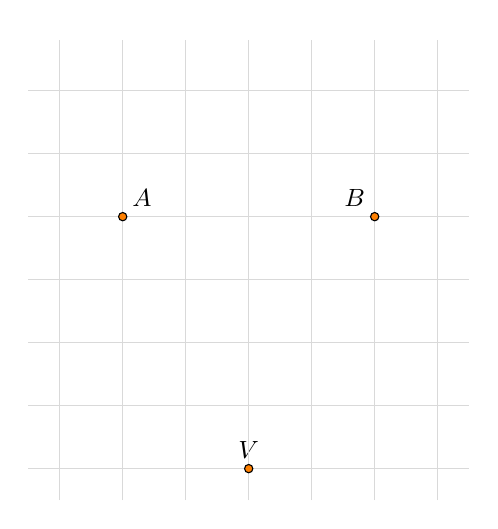
\begin{tikzpicture}[x=8mm, y=8mm,font=\small]

  \node[above right] at (-1,0) {$A$};
  \node[above left] at (3,0) {$B$};
  \node[above] at (1,-4) {$V$};
  \draw[step=0.8cm,color=gray!30] (-2.5,-4.5) grid (4.5,2.8);
  \tkzInit[xmin=-2,xmax=3.5,ymin=-4.5,ymax=2.2]
  \clip (-2.5,-4.3) rectangle (4.5,3);
  \begin{scope}[font=\small]
    \tkzAxeY[orig = false, label options={left = 1pt}]
    \tkzAxeX[orig = true, label options={below = 1pt}]
  \end{scope}
  \tkzFct[domain=-1.5:3.5,thick,color=Maroon]{x*x-2*x-3};
  \draw[fill=orange] (-1,0)circle (1.5pt);
  \draw[fill=orange] (3,0)circle (1.5pt);
  \draw[fill=orange] (1,-4)circle (1.5pt);

\end{tikzpicture}

\end{center}
\end{esempio}
\end{exrig}
\vspazio\ovalbox{\risolvii \ref{ese:4.6}, \ref{ese:4.7}}

\subsection{Segno di un trinomio di secondo grado per via grafica}

\begin{exrig}
\begin{esempio}
Studiare il segno del trinomio $x^2-2x-3$.

Si tratta di stabilire per quali valori di $x$ esso assume segno positivo, per quali segno negativo e per quali eventualmente si annulla.

La richiesta è interpretabile anche come la ricerca degli insiemi soluzioni dell'equazione $x^2-2x-3=0$ e delle disequazioni $x^2-2x-3>0$ e $x^2-2x-3<0$.

\emph{Strategia risolutiva}:
Tracciamo il grafico della funzione $y=x^2-2x-3$ e leggiamo dal grafico gli insiemi richiesti (vedi la figura precedente):
\begin{itemize}
\item Le ascisse dei punti $A$ e $B$ costituiscono l'insieme soluzione dell'equazione $x^2-2x-3=0$ cioè $x_1=-1\vee x_2=3$;
\item I valori di $x$ dell'insieme $H=\{x\in \insR \mid x_A<x<x_B\}$ rendono il trinomio negativo; infatti preso un valore dell'insieme, ad esempio $x=0$, il punto sulla parabola ha ordinata negativa $(-3)$. Per esercizio segnate il punto sul grafico e ripetete per $x=1$, $x=\frac 3 2$, $x=2$;
\item I valori di $x$ dell'insieme $K=\{x\in \insR \mid x<x_A\vee x>x_B\}$ rendono il trinomio positivo; infatti preso un valore dell'insieme, ad esempio $x=\frac 7 2$, il punto sulla parabola ha ordinata positiva. Per esercizio segnatelo sul grafico e ripetete per $x=-\frac{6}{5}$.
\end{itemize}
\end{esempio}
\end{exrig}
\osservazione La ricerca dell'insieme soluzione di una disequazione di secondo grado è sempre interpretabile come la ricerca del segno di un trinomio di secondo grado e quindi risolubile per via grafica. In questi casi non è necessario rappresentare in modo preciso la parabola associata al trinomio, ma basta ricordare quanto detto inizialmente sugli zeri di una funzione (vedi la figura~\ref{fig:subfig10} a pagina~\pageref{fig:subfig10}).

\begin{figure}[tp]
\centering
% (c) 2013 Claudio Carboncini - claudio.carboncini@gmail.com
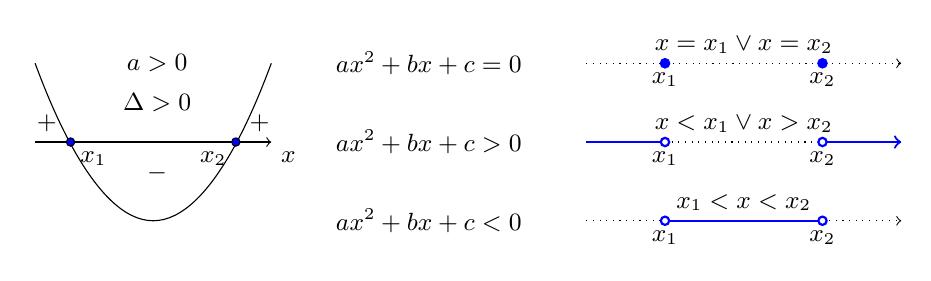
\begin{tikzpicture}[font=\small,x=10mm, y=10mm]

% prima parabola;
  \draw (-1,0) parabola[parabola height=-2cm] +(3,0);
  \draw[->] (-1,-1) -- (2,-1) node [below right] () {$x$};
  \draw[fill=blue] (-.55,-1)circle (1.5pt);
  \draw[fill=blue] (1.55,-1)circle (1.5pt);
  \node[below right] at (-.55,-1) {$x_1$};
  \node[below left] at (1.55,-1) {$x_2$};
  \node[above right] at (1.6,-1) {$+$};
  \node[above left] at (-.6,-1) {$+$};
  \node[] at (.55,-1.4) {$-$};
  \node[] at (.55,-.50) {$\Delta>0$};
  \node[] at (.55,0) {$a>0$};
%segno
  \node[] at (4,0) {$ax^2+bx+c=0$};
  \node[] at (4,-1) {$ax^2+bx+c>0$};
  \node[] at (4,-2) {$ax^2+bx+c<0$};

%Insieme soluzione
%primo insieme
\begin{scope}[dotted]
\draw[->] (6,0) -- (10,0);
\end{scope}
\node[below]  at (7,0) {$x_1$};
\node[below]  at (9,0) {$x_2$};
\node[above]  at (8,0) {$x=x_1 \vee x=x_2$};
\begin{scope}[blue,thick]
\draw[fill=blue] (7,0)circle (1.5pt);
\draw[fill=blue] (9,0)circle (1.5pt);
\end{scope}
%secondo insieme
\begin{scope}[dotted]
\draw (7,-1) -- (9,-1);
\end{scope}
\node[below]  at (7,-1) {$x_1$};
\node[below]  at (9,-1) {$x_2$};
\node[above]  at (8,-1) {$x<x_1 \vee x>x_2$};
\begin{scope}[blue,thick]
\draw (6,-1) -- (7,-1);
\draw[->] (9,-1) -- (10,-1);
\draw[fill=white] (7,-1)circle (1.5pt);
\draw[fill=white] (9,-1)circle (1.5pt);
\end{scope}

%terzo insieme
\begin{scope}[dotted]
\draw (6,-2) -- (7,-2);
\draw[->] (9,-2) -- (10,-2);
\end{scope}
\node[below]  at (7,-2) {$x_1$};
\node[below]  at (9,-2) {$x_2$};
\begin{scope}[blue,thick]
\draw (7,-2) -- (9,-2);
\draw[fill=white] (7,-2)circle (1.5pt);
\draw[fill=white] (9,-2)circle (1.5pt);
\end{scope}
\node[above]  at (8,-2) {$x_1<x<x_2$};

\end{tikzpicture}


\vspace{12pt}
{% (c) 2013 Claudio Carboncini - claudio.carboncini@gmail.com
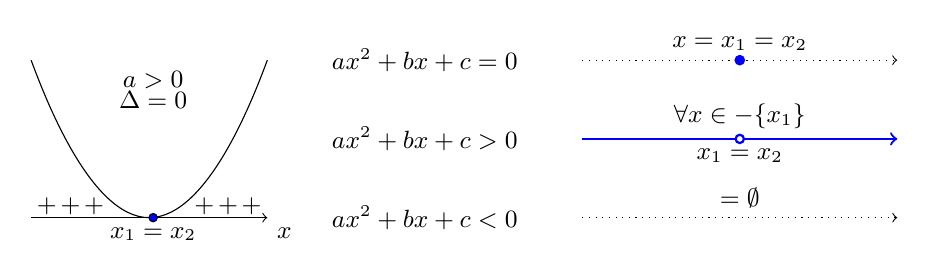
\begin{tikzpicture}[font=\small,x=10mm, y=10mm]

% seconda parabola;
  \draw (-1,0) parabola[parabola height=-2cm] +(3,0);
  \draw[->] (-1,-2) -- (2,-2) node [below right] () {$x$};
  \draw[fill=blue] (.55,-2)circle (1.5pt);
  \foreach \x in {-.8,-.5,-.2,1.2,1.5,1.8}{
  \node  at (\x,-1.85) {$+$};
  }
  \node[below] at (.55,-2) {$x_1=x_2$};
  \node[] at (.55,-.5) {$\Delta=0$};
  \node[] at (.55,-.25) {$a>0$};
%segno
  \node[] at (4,0) {$ax^2+bx+c=0$};
  \node[] at (4,-1) {$ax^2+bx+c>0$};
  \node[] at (4,-2) {$ax^2+bx+c<0$};
%Insieme soluzione

%primo insieme
\begin{scope}[dotted]
\draw (6,0) -- (8,0);
\draw[->] (8,0) -- (10,0);
\end{scope}
\node[above]  at (8,0) {$x=x_1=x_2$};
\begin{scope}[blue,thick]
\draw[fill=blue] (8,0)circle (1.5pt);
\end{scope}

%secondo insieme
\node[below]  at (8,-1) {$x_1=x_2$};
\node[above]  at (8,-1) {$\forall{x} \in \insR-\{x_1\}$};
\begin{scope}[blue,thick]
\draw[->] (6,-1) -- (10,-1);
\draw[fill=white] (8,-1)circle (1.5pt);
\end{scope}

%terzo insieme
\begin{scope}[dotted]
\draw[->] (6,-2) -- (10,-2);
\end{scope}
\node[above]  at (8,-2) {$\IS=\emptyset$};

\end{tikzpicture}

}
\vspace{12pt}
{% (c) 2013 Claudio Carboncini - claudio.carboncini@gmail.com
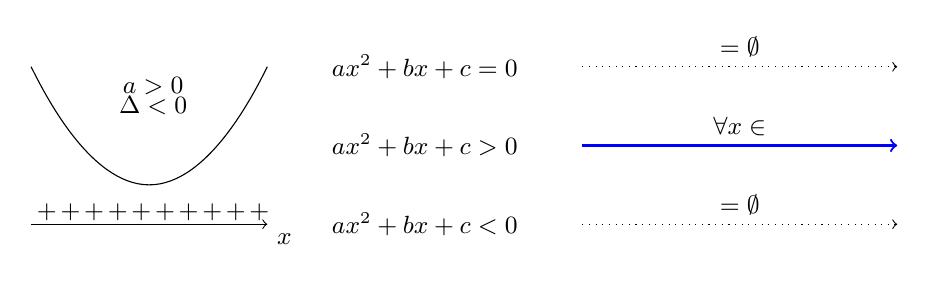
\begin{tikzpicture}[font=\small,x=10mm, y=10mm]

% terza parabola;
  \draw (-1,0) parabola[parabola height=-1.5cm] +(3,0);
  \draw[->] (-1,-2) -- (2,-2) node [below right] () {$x$};
  \foreach \x in {-.8,-.5,-.2,.1,.4,.7,1,1.3,1.6,1.9}{
  \node  at (\x,-1.85) {$+$};
  }
  \node[] at (.55,-.5) {$\Delta<0$};
  \node[] at (.55,-.25) {$a>0$};
%segno
  \node[] at (4,0) {$ax^2+bx+c=0$};
  \node[] at (4,-1) {$ax^2+bx+c>0$};
  \node[] at (4,-2) {$ax^2+bx+c<0$};
%Insieme soluzione
%primo insieme
\begin{scope}[dotted]
\draw[->] (6,0) -- (10,0);
\end{scope}
\node[above]  at (8,0) {$\IS=\emptyset$};
%secondo insieme
\node[above]  at (8,-1) {$\forall x \in \insR$};
\begin{scope}[blue,thick]
\draw[->] (6,-1) -- (10,-1);
\end{scope}
%terzo insieme
\begin{scope}[dotted]
\draw[->] (6,-2) -- (10,-2);
\end{scope}
\node[above]  at (8,-2) {$\IS=\emptyset$};

\end{tikzpicture}

}
\vspace{12pt}
{% (c) 2013 Claudio Carboncini - claudio.carboncini@gmail.com
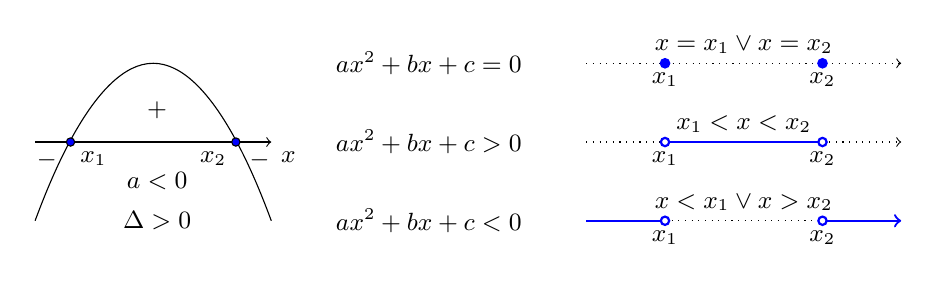
\begin{tikzpicture}[font=\small,x=10mm, y=10mm]

% prima parabola;
  \draw (-1,0) parabola[parabola height=2cm] +(3,0);
  \draw[->] (-1,1) -- (2,1) node [below right] () {$x$};
  \draw[fill=blue] (-.55,1)circle (1.5pt);
  \draw[fill=blue] (1.55,1)circle (1.5pt);
  \node[below right] at (-.55,1) {$x_1$};
  \node[below left] at (1.55,1) {$x_2$};
  \node[below right] at (1.6,1) {$-$};
  \node[below left] at (-.6,1) {$-$};
  \node[] at (.55,1.4) {$+$};
  \node[] at (.55,0) {$\Delta>0$};
  \node[] at (.55,.5) {$a<0$};
%segno
  \node[] at (4,2) {$ax^2+bx+c=0$};
  \node[] at (4,1) {$ax^2+bx+c>0$};
  \node[] at (4,0) {$ax^2+bx+c<0$};

%Insieme soluzione
%primo insieme
\begin{scope}[dotted]
\draw[->] (6,2) -- (10,2);
\end{scope}
\node[below]  at (7,2) {$x_1$};
\node[below]  at (9,2) {$x_2$};
\node[above]  at (8,2) {$x=x_1 \vee x=x_2$};
\begin{scope}[blue,thick]
\draw[fill=blue] (7,2)circle (1.5pt);
\draw[fill=blue] (9,2)circle (1.5pt);
\end{scope}
%secondo insieme
\begin{scope}[dotted]
\draw (6,1) -- (7,1);
\draw[->] (9,1) -- (10,1);
\end{scope}
\node[below]  at (7,1) {$x_1$};
\node[below]  at (9,1) {$x_2$};
\node[above]  at (8,1) {$x_1<x<x_2$};
\begin{scope}[blue,thick]
\draw (7,1) -- (9,1);
\draw[fill=white] (7,1)circle (1.5pt);
\draw[fill=white] (9,1)circle (1.5pt);
\end{scope}

%terzo insieme
\begin{scope}[dotted]
\draw (7,0) -- (9,0);
\end{scope}
\node[below]  at (7,0) {$x_1$};
\node[below]  at (9,0) {$x_2$};
\begin{scope}[blue,thick]
\draw (6,0) -- (7,0);
\draw[->] (9,0) -- (10,0);
\draw[fill=white] (7,0)circle (1.5pt);
\draw[fill=white] (9,0)circle (1.5pt);
\end{scope}
\node[above]  at (8,0) {$x<x_1 \vee x>x_2$};

\end{tikzpicture}

}
\vspace{12pt}
{% (c) 2013 Claudio Carboncini - claudio.carboncini@gmail.com
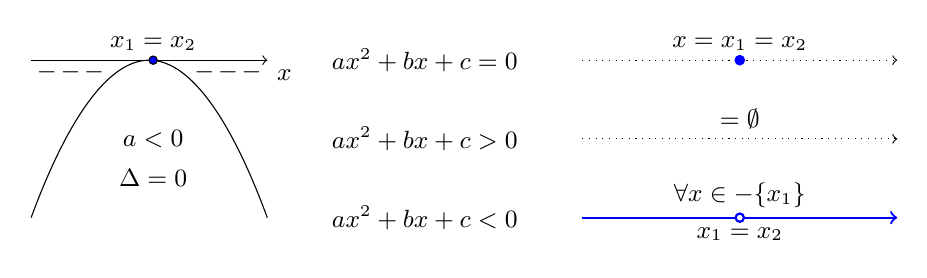
\begin{tikzpicture}[font=\small,x=10mm, y=10mm]

% quarta parabola;
  \draw (-1,0) parabola[parabola height=2cm] +(3,0);
  \draw[->] (-1,2) -- (2,2) node [below right] () {$x$};
  \draw[fill=blue] (.55,2)circle (1.5pt);
  \foreach \x in {-.8,-.5,-.2,1.2,1.5,1.8}{
  \node  at (\x,1.85) {$-$};
  }
  \node[above] at (.55,2) {$x_1=x_2$};
  \node[] at (.55,.5) {$\Delta=0$};
  \node[] at (.55,1) {$a<0$};
%segno
  \node[] at (4,2) {$ax^2+bx+c=0$};
  \node[] at (4,1) {$ax^2+bx+c>0$};
  \node[] at (4,0) {$ax^2+bx+c<0$};
%Insieme soluzione

%primo insieme
\begin{scope}[dotted]
\draw (6,2) -- (8,2);
\draw[->] (8,2) -- (10,2);
\end{scope}
\node[above]  at (8,2) {$x=x_1=x_2$};
\begin{scope}[blue,thick]
\draw[fill=blue] (8,2)circle (1.5pt);
\end{scope}

%secondo insieme
\begin{scope}[dotted]
\draw[->] (6,1) -- (10,1);
\end{scope}
\node[above]  at (8,1) {$\IS=\emptyset$};

%terzo insieme
\node[below]  at (8,0) {$x_1=x_2$};
\node[above]  at (8,0) {$\forall x \in \insR-\{x_1\}$};
\begin{scope}[blue,thick]
\draw[->] (6,0) -- (10,0);
\draw[fill=white] (8,0)circle (1.5pt);
\end{scope}

\end{tikzpicture}

}
\vspace{12pt}
{% (c) 2013 Claudio Carboncini - claudio.carboncini@gmail.com
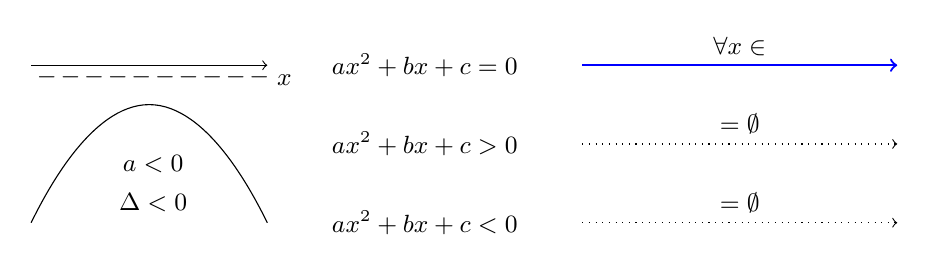
\begin{tikzpicture}[font=\small,x=10mm, y=10mm]

% ultima parabola;
  \draw (-1,0) parabola[parabola height=1.5cm] +(3,0);
  \draw[->] (-1,2) -- (2,2) node [below right] () {$x$};
  \foreach \x in {-.8,-.5,-.2,.1,.4,.7,1,1.3,1.6,1.9}{
  \node  at (\x,1.85) {$-$};
  }
  \node[] at (.55,.25) {$\Delta<0$};
  \node[] at (.55,.75) {$a<0$};
%segno
  \node[] at (4,2) {$ax^2+bx+c=0$};
  \node[] at (4,1) {$ax^2+bx+c>0$};
  \node[] at (4,0) {$ax^2+bx+c<0$};
%Insieme soluzione
%primo insieme
\begin{scope}[blue,thick]
\draw[->] (6,2) -- (10,2);
\end{scope}
\node[above]  at (8,2) {$\forall x \in \insR$};
%secondo insieme
\begin{scope}[dotted]
\draw[->] (6,0) -- (10,0);
\end{scope}
\node[above]  at (8,0) {$\IS=\emptyset$};
%terzo insieme
\begin{scope}[dotted]
\draw[->] (6,1) -- (10,1);
\end{scope}
\node[above]  at (8,1) {$\IS=\emptyset$};

\end{tikzpicture}

}
\caption{Risoluzione delle disequazioni di secondo grado}
\label{fig:subfig10}
\end{figure}

\begin{exrig}
\begin{esempio}
Risolvi le seguenti disequazioni utilizzando il segno del trinomio di secondo grado.
\begin{itemize}
\item $x^2+x-2>0$.

Risolviamo l'equazione $x^2+x-2=0$ che avendo il discriminante positivo ammette due soluzioni reali distinte $x_1=-2\vee x_2=1$. Tali valori sono gli zeri del trinomio e dunque gli zeri della funzione $y=x^2+x-2$; la parabola volge la concavità verso l'alto quindi possiamo grossolanamente rappresentare la sua posizione rispetto all'asse $x$ e dedurre l'insieme soluzione richiesto: $\IS=\{x\in \insR \mid x<-2\vee x>1\}$ o con notazione insiemistica $(-\infty$, $-2)\cup (1$, $+\infty)$;
\item $x^2-4x+4\le 0$.

Risolviamo l'equazione $x^2-4x+4=0$ che avendo il discriminante nullo ammette due soluzioni reali coincidenti $x_1=x_2=2$: gli zeri del trinomio sono quindi coincidenti nel numero $2$; la parabola $y=x^2-4x+4$ ha il vertice sull'asse $x$ e volge la concavità verso l'alto quindi possiamo grossolanamente rappresentare la sua posizione e dedurre l'insieme soluzione richiesto: $\IS=\{x\in \insR \mid x=2\}$, ovvero $\{2\}$. Nessun valore reale rende il trinomio negativo;
\item $x^2-2x+7>0$.

Risolviamo l'equazione $x^2-2x+7=0$ che avendo il discriminante negativo non ammette soluzioni reali; il trinomio non ha zeri reali, la parabola $y=x^2-2x+7$ volge la concavità verso l'alto e non ha punti appartenenti all'asse $x$ quindi possiamo grossolanamente rappresentare la sua posizione e dedurre l'insieme soluzione richiesto: $\IS=\insR$, ovvero $(-\infty$, $+\infty)$.
\end{itemize}
\begin{center}
 % (c) 2013 Claudio Carboncini - claudio.carboncini@gmail.com
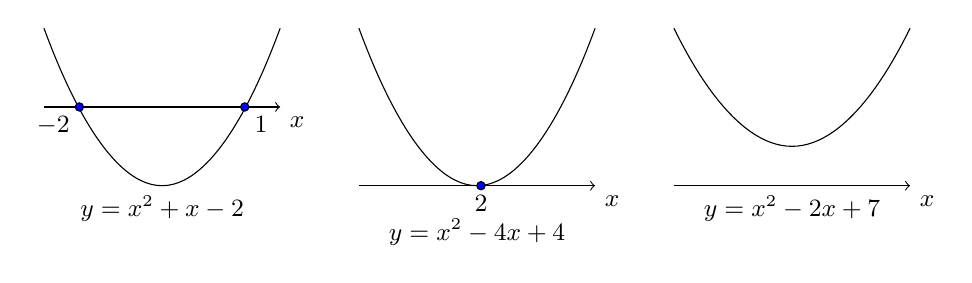
\begin{tikzpicture}[font=\small,x=10mm, y=10mm]
% prima parabola;
  \draw (-1,0) parabola[parabola height=-2cm] +(3,0);
  \draw[->] (-1,-1) -- (2,-1) node [below right] () {$x$};
  \draw[fill=blue] (-.55,-1)circle (1.5pt);
  \draw[fill=blue] (1.55,-1)circle (1.5pt);
  \node[below left] at (-.55,-1) {$-2$};
  \node[below right] at (1.55,-1) {$1$};
  \node[below] at(.5,-2) {$y=x^2+x-2$};
%seconda parabola
  \draw (3,0) parabola[parabola height=-2cm] +(3,0);
  \draw[->] (3,-2) -- (6,-2) node [below right] () {$x$};
  \draw[fill=blue] (4.55,-2)circle (1.5pt);
  \node[below] at (4.55,-2) {$2$};
  \node[below] at(4.5,-2.3) {$y=x^2-4x+4$};
 % terza parabola;
  \draw (7,0) parabola[parabola height=-1.5cm] +(3,0);
  \draw[->] (7,-2) -- (10,-2) node [below right] () {$x$};
  \node[below] at(8.5,-2) {$y=x^2-2x+7$};
\end{tikzpicture}


\end{center}
\end{esempio}
\end{exrig}
\vspazio\ovalbox{\risolvii \ref{ese:4.8}, \ref{ese:4.9}, \ref{ese:4.10}, \ref{ese:4.11}, \ref{ese:4.12}, \ref{ese:4.13}, \ref{ese:4.14}, \ref{ese:4.15}, \ref{ese:4.16}, \ref{ese:4.17}, \ref{ese:4.18}, \ref{ese:4.19}, \ref{ese:4.20},}

\vspazio\ovalbox{ \ref{ese:4.21}, \ref{ese:4.22}, \ref{ese:4.23}}
\pagebreak
\section{Segno del trinomio a coefficienti letterali}

Consideriamo il trinomio $t=kx^2+3x-7$ avente il coefficiente del termine di secondo grado dipendente dal parametro $k$.

Come possiamo stabilire il segno del trinomio~$t=kx^2+3x-7$, al variare di $k$?
Sappiamo che stabilire il segno di un trinomio significa determinare i valori reali che attribuiti alla variabile indipendente $x$ rendono il trinomio positivo, nullo o negativo. Evidentemente per i vari valori reali di $k$ avremo una diversa disequazione da risolvere; dobbiamo dunque cercare di analizzare come varia il trinomio al variare dei valori di $k$ e in seguito studiare il segno del trinomio ottenuto.

Questa analisi di situazioni diverse è la \textit{discussione del trinomio a coefficienti parametrici}.

\begin{exrig}
\begin{esempio}
Stabilire il segno di $t=kx^2+3x-7$ al variare di $ k $.

Prendiamo in considerazione il segno del coefficiente del termine di secondo grado e il segno del discriminante dell'equazione associata $kx^2+3x-7=0$. Il coefficiente del termine di secondo grado è maggiore di zero per $k>0$. Il discriminante $\Delta =9+28k$ è positivo per $k>-\frac 9{28}$. Rappresentiamo la loro reciproca situazione:
\begin{center}
 % (c) 2013 Claudio Carboncini - claudio.carboncini@gmail.com
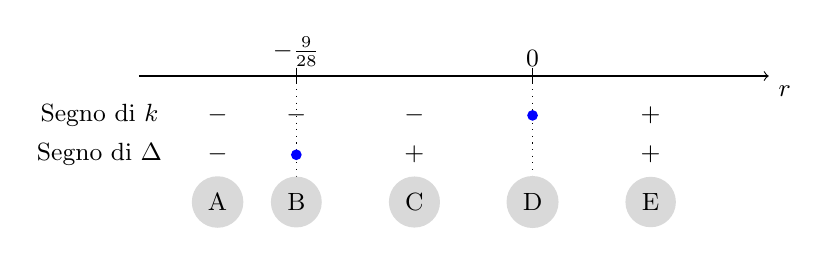
\begin{tikzpicture}[font=\small,x=10mm, y=10mm]

\draw[->] (0,0) -- (8,0) node [below right] () {$r$};

\foreach \x in {2,5}{
\draw(\x,3pt)--(\x,-3pt);
\begin{scope}[dotted]
\draw (\x,0) -- (\x,-1.5);
\end{scope}}
\node[] at (-.5,-0.5) {Segno di $k$};
\node[] at (-.5,-1) {Segno di $\Delta$};
\node[above]  at (2,0) {$-\frac{9}{28}$};
\node[above]  at (5,0) {$0$};
\node[] at (1,-0.5) {$-$};
\node[] at (2,-0.5) {$-$};
\node[] at (3.5,-0.5) {$-$};
\node[] at (6.5,-0.5) {$+$};
\node[] at (1,-1) {$-$};
\node[] at (3.5,-1) {$+$};
\node[] at (6.5,-1) {$+$};
\node [circle,fill=gray!30](A) at (1,-1.6) {A};
\node [circle,fill=gray!30](B) at (2,-1.6) {B};
\node [circle,fill=gray!30](C) at (3.5,-1.6) {C};
\node [circle,fill=gray!30](D) at (5,-1.6) {D};
\node [circle,fill=gray!30](E) at (6.5,-1.6) {E};

\begin{scope}[blue,thick]
\draw[fill=blue] (5,-.5)circle (1.5pt);
\draw[fill=blue] (2,-1)circle (1.5pt);
\end{scope}

\end{tikzpicture}

\end{center}
\begin{enumerate}[label=(\Alph*)]
\item $k<-\frac 9{28}$: il coefficiente del termine di secondo grado è negativo così come il discriminante, la parabola volge la concavità verso il basso e non ha zeri reali: il trinomio è negativo per qualunque valore reale di $x$;
\item $k=-\frac 9{28}$: il coefficiente del termine di secondo grado è negativo e il discriminante è uguale a zero. La parabola volge la concavità verso il basso e ha due zeri reali coincidenti $x_1=x_2=\frac{14} 3$. Il trinomio si annulla per $x=\frac{14} 3$ mentre per qualunque altro valore di $x$ è negativo;
\item $-\frac 9{28}<k<0$: il coefficiente del termine di secondo grado è negativo e il discriminante è positivo. La parabola volge la concavità verso il basso e ha due zeri reali distinti: il trinomio si annulla per $x=x_1\vee x=x_2$; è positivo per $x_1<x<x_2$; è negativo per $x<x_1\vee x>x_2$;
\item $k=0$: il trinomio diventa un binomio di primo grado: $t=3x-7$ e quindi $t>0$ per $x>\frac 7 3$, $t<0$ per $x<\frac 7 3$, $t=0$ per $x=\frac 7 3$;
\item $k>0$: Il coefficiente del termine di secondo grado è positivo così come il discriminante. La parabola ha concavità verso l'alto e due zeri reali distinti: il trinomio si annulla per $x=x_1\vee x=x_2$; è negativo per $x_1<x<x_2$; è positivo per $x<x_1\vee x>x_2$\emph{.}
\end{enumerate}
\end{esempio}
\pagebreak
\begin{esempio}
Stabilite al variare del parametro $k$ l'insieme soluzione della disequazione $x^2+kx+1<0$.

Prendiamo in considerazione il primo coefficiente (quello del termine di secondo grado) e il discriminante dell'equazione associata $x^2+kx+1=0$ e stabiliamo il loro segno: il primo coefficiente è 1 e quindi indipendente dal parametro e sempre positivo quindi la parabola volge sempre la concavità verso l'alto. Essendo il discriminante $\Delta =k^2-4$ si hanno soluzioni reali per $k\le -2\vee k\ge 2$. Rappresentiamo la loro reciproca situazione:
\begin{center}
 % (c) 2013 Claudio Carboncini - claudio.carboncini@gmail.com
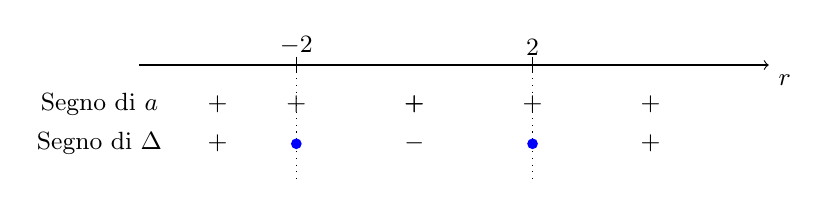
\begin{tikzpicture}[font=\small,x=10mm, y=10mm]

\draw[->] (0,0) -- (8,0) node [below right] () {$r$};

\foreach \x in {2,5}{
\draw(\x,3pt)--(\x,-3pt);
\begin{scope}[dotted]
\draw (\x,0) -- (\x,-1.5);
\end{scope}}
\node[] at (-.5,-0.5) {Segno di $a$};
\node[] at (-.5,-1) {Segno di $\Delta$};
\node[above]  at (2,0) {$-2$};
\node[above]  at (5,0) {$2$};
\node[] at (1,-0.5) {$+$};
\node[] at (2,-0.5) {$+$};
\node[] at (3.5,-0.5) {$+$};
\node[] at (3.5,-0.5) {$+$};
\node[] at (5,-0.5) {$+$};
\node[] at (6.5,-0.5) {$+$};
\node[] at (1,-1) {$+$};
\node[] at (3.5,-1) {$-$};
\node[] at (6.5,-1) {$+$};

\begin{scope}[blue,thick]
\draw[fill=blue] (5,-1)circle (1.5pt);
\draw[fill=blue] (2,-1)circle (1.5pt);
\end{scope}

\end{tikzpicture}

\end{center}
\begin{itemize*}
\item $k<-2\vee k>2$; il discriminante è positivo. L'equazione ha due zeri reali distinti: $x=x_1\vee x=x_2$ quindi $\IS=\{x \in \insR \mid x_1<x<x_2\}$;
\item $-2<k<2$; il discriminante è negativo. La parabola non ha zeri reali: $\IS=\emptyset$;
\item $k=-2\vee k=2$; il discriminante è nullo. In ognuno dei due casi la parabola ha un unico zero reale: $\IS=\{-1$, $1\}$.
\end{itemize*}
\end{esempio}
\end{exrig}

\vspazio\ovalbox{\risolvii \ref{ese:4.24}, \ref{ese:4.25}, \ref{ese:4.26}}

\section{Disequazioni polinomiali di grado superiore al secondo}

\begin{exrig}
\begin{esempio}
Un numero è tale che sottraendo al suo cubo il suo triplo si ottiene un valore maggiore del triplo del suo quadrato aumentato di $4$. Qual è il numero cercato?

La richiesta del problema implica la ricerca dell'insieme soluzione della disequazione $x^3-3x>3x^2+4$ di terzo grado nella variabile $x$. Scriviamo la disequazione in forma canonica, applicando i principi di equivalenza: $x^3-3x^2-3x-4>0$. Si tratta di una disequazione polinomiale di terzo grado.

Procediamo nella scomposizione in fattori del polinomio $p(x)=x^3-3x^2-3x-4$. Mediante la regola di Ruffini possiamo determinare un suo zero $x=4$ e dunque ottenere $p(x)=(x-4)(x^2+x+1)$.

Determiniamo il segno dei singoli fattori: il primo fattore $f_1=x-4>0\:\Rightarrow\: x>4$; il secondo fattore $f_2=x^2+x+1>0$ è una disequazione di secondo grado. Il primo coefficiente è positivo, quindi la parabola volge la concavità verso l'alto, e il discriminante $\Delta =1-4=-3$ è negativo, pertanto l'equazione associata non ha zeri reali, dunque $f_2$ è positivo per qualunque valore reale di $x$. Costruiamo la tabella dei segni:
\begin{center}
 % (c) 2013 Claudio Carboncini - claudio.carboncini@gmail.com
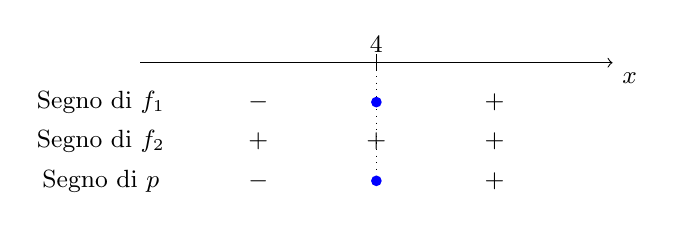
\begin{tikzpicture}[font=\small,x=10mm, y=10mm]

\draw[->] (0,0) -- (6,0) node [below right] () {$x$};

\draw(3,3pt)--(3,-3pt);
\begin{scope}[dotted]
\draw (3,0) -- (3,-1.5);
\end{scope}
\node[] at (-.5,-0.5) {Segno di $f_1$};
\node[] at (-.5,-1) {Segno di $f_2$};
\node[] at (-.5,-1.5) {Segno di $p$};
\node[above]  at (3,0) {$4$};
\node[] at (1.5,-0.5) {$-$};
\node[] at (4.5,-0.5) {$+$};
\node[] at (1.5,-1) {$+$};
\node[] at (3,-1) {$+$};
\node[] at (4.5,-1) {$+$};
\node[] at (1.5,-1.5) {$-$};
\node[] at (4.5,-1.5) {$+$};

\begin{scope}[blue,thick]
\draw[fill=blue] (3,-1.5)circle (1.5pt);
\draw[fill=blue] (3,-.5)circle (1.5pt);
\end{scope}

\end{tikzpicture}

\end{center}
$\IS=\{x\in \insR \mid x>4\}=(4$, $+\infty)$.
\end{esempio}
\end{exrig}

\begin{procedura}
Risolvere le disequazioni di grado superiore al primo:
\begin{enumeratea}
\item scomporre il polinomio di grado $n$ in fattori di primo e secondo grado;
\item studiare il segno dei singoli fattori;
\item costruire la tabella dei segni;
\item cercare gli intervalli in cui il polinomio dato assume il segno richiesto.
\end{enumeratea}
\end{procedura}

\begin{exrig}
\begin{esempio}
$-2x(3-2x)-3x^2\left(2-\dfrac 3 2x\right)\ge 5\left(2x^2-\dfrac 3{10}x\right)$.

Osserviamo che la disequazione proposta è polinomiale di terzo grado; eseguiamo i calcoli per portarla alla forma $p(x)\ge 0$. Si ottiene $3x^3-8x^2-3x\ge 0$ e con la scomposizione si ha $x\cdot (3x^2-8x-3)\ge 0$. Procediamo con lo studio dei segni dei singoli fattori: $f_1=x\ge 0$ e $f_2=3x^2-8x-3\ge 0 \:\Rightarrow\: x\le -\frac 1 3\vee x\ge 3$ e compiliamo la tabella dei segni, che lasciamo fare al lettore.
\begin{center}
 % (c) 2013 Claudio Carboncini - claudio.carboncini@gmail.com
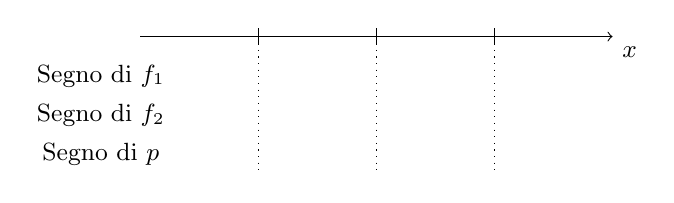
\begin{tikzpicture}[font=\small,x=10mm, y=10mm]

\draw[->] (0,0) -- (6,0) node [below right] () {$x$};

\foreach \x in {1.5,3,4.5}{
\draw(\x,3pt)--(\x,-3pt);
\begin{scope}[dotted]
\draw (\x,0) -- (\x,-1.7);
\end{scope}}
\node[] at (-.5,-0.5) {Segno di $f_1$};
\node[] at (-.5,-1) {Segno di $f_2$};
\node[] at (-.5,-1.5) {Segno di $p$};

\end{tikzpicture}

\end{center}
Otteniamo: $\IS=\left\{x\in \insR \mid -\frac 1 3\le x\le 0\vee x\ge 3\right\}$.
\end{esempio}

\begin{esempio}
$64x^6-1<0$.

Il binomio al primo membro è una differenza di quadrati, quindi scomponendolo si ottiene: $64x^6-1=(8x^3-1)(8x^3+1)=(2x-1)(4x^2+2x+1)(2x+1)(4x^2-2x+1)$.

Si tratta allora di studiare il segno dei singoli fattori: $f_1=2x-1>0\:\Rightarrow\: x>\frac 1 2$; $f_2=4x^2+2x+1>0\:\Rightarrow\: \forall x\in \insR$; $f_3=2x+1>0\:\Rightarrow\: x>-\frac 1 2$; $f_4=4x^2-2x+1>0\:\Rightarrow\: \forall x\in \insR$ e di determinare il segno richiesto dopo aver costruito la tabella dei segni.
\end{esempio}

\begin{esempio}
$x^4-4x^2-45>0$.

Il trinomio al primo membro è di quarto grado; sappiamo che con la sostituzione $x^2=t$ può essere ricondotto ad un trinomio di secondo grado la cui scomposizione in fattori risulta $(t-9)\cdot (t+5)$ e quindi la disequazione assegnata diventa: $(x^2-9)\cdot (x^2+5)>0$.

Si tratta allora di studiare il segno dei singoli fattori $f_1=x^2-9>0\:\Rightarrow\: x<-3\vee x>3$ e $f_2=x^2+5>0\:\Rightarrow\: \forall x\in \insR$ per poi determinare il segno richiesto dopo aver costruito la tabella dei segni.
\end{esempio}
\end{exrig}
\vspazio\ovalbox{\risolvii \ref{ese:4.27}, \ref{ese:4.28}, \ref{ese:4.29}, \ref{ese:4.30}, \ref{ese:4.31}, \ref{ese:4.32}, \ref{ese:4.33}, \ref{ese:4.34}, \ref{ese:4.35}, \ref{ese:4.36}, \ref{ese:4.37}, \ref{ese:4.38}, \ref {ese:4.39},}

\vspazio\ovalbox{\ref{ese:4.40}, \ref{ese:4.41}, \ref{ese:4.42}, \ref{ese:4.43}, \ref{ese:4.44}, \ref{ese:4.45}, \ref{ese:4.46}, \ref{ese:4.47}, \ref{ese:4.48}, \ref{ese:4.49}, \ref{ese:4.50}}
\pagebreak
\section{Disequazioni fratte}

Ricordiamo che una disequazione è \emph{frazionaria} o \emph{fratta} quando il suo denominatore contiene l'incognita.
\begin{procedura}
Soluzione di una disequazione frazionaria:
\begin{enumeratea}
\item applicando il primo principio di equivalenza si trasportano tutti i termini al primo membro e si calcola il risultato dell'equazione assegnata $E(x)=\frac{N(x)}{D(x)}$;
\item si determinano le condizioni di esistenza ponendo $D(x)\neq 0$;
\item impostiamo la disequazione nella forma $\frac{N(x)}{D(x)}\ge 0$, $\frac{N(x)}{D(x)}\le 0$, $\frac{N(x)}{D(x)}>0$ o $\frac{N(x)}{D(x)}<0$ a seconda del quesito posto da problema;
\item si studia il segno del numeratore e del denominatore, ponendo $N(x)>0$ oppure $N(x)\ge 0$ (a seconda della richiesta) e $D(x)>0$;
\item si costruisce la tabella dei segni, segnando con un punto pieno gli zeri della frazione, se richiesti;
\item si individuano gli intervalli in cui la frazione assume il segno richiesto.
\end{enumeratea}
\end{procedura}

Vediamo attraverso alcuni esempi come procedere.
\begin{exrig}
\begin{esempio}
Data l'espressione $E=\dfrac 4{4x^2-1}+\dfrac 1{2x+1}+\dfrac x{1-2x}$ determinarne, al variare di $x$ in $\insR$, il segno.

\emph{Osservazioni preliminari}
\begin{itemize*}
\item L'espressione assegnata è frazionaria, quindi lo studio del segno deve essere circoscritto ai valori di $x$ del dominio $\Dom$ dell'espressione stessa;
\item studiare il segno di una espressione letterale significa stabilire in quale insieme si trovano i valori della variabile che la rendono positiva, negativa, nulla;
\item ogni espressione contenente operazioni tra frazioni algebriche ha in generale come risultato una frazione algebrica.
\end{itemize*}

\emph{Strategia risolutiva}
\begin{enumeratea}
\item semplifichiamo l'espressione assegnata: $E=\frac{-2x^2+x+3}{(2x+1)\cdot (2x-1)}$;
\item determiniamo il dominio: $\CE\, 2x+1\neq 0\;\wedge\; 2x-1\neq 0\:\Rightarrow\: \Dom=\insR-\left\{-\frac 1 2\text{, }\frac 1 2\right\}$;
\item impostiamo la disequazione: $\frac{-2x^2+x+3}{(2x+1)\cdot (2x-1)}\ge 0$ che ci permetterà di rispondere al quesito posto dal problema;
\item studiamo il segno di numeratore $N$ e denominatore $D$:
 \begin{itemize*}
\item segno di $N$: $-2x^2+x+3\ge 0$ disequazione di secondo grado, quindi dall'equazione associata $-2x^2+x+3=0$, calcoliamo il discriminante: $\Delta =1+24=25$, positivo per cui si hanno due soluzioni reali distinte; la parabola $y=-2x^2+x+3$ ha concavità verso il basso, per cui essendo $x_1=-1$ e $x_2=\frac 3 2$ si ha $N\ge 0$ per $-1\le x\le \frac 3 2$;
\item segno di $D$: il denominatore è composto da due fattori di primo grado $d_1$ e $d_2$, quindi $d_1>0$ per $x>-\frac 1 2$ e $d_2>0$ per $x>\frac 1 2$;
 \end{itemize*}
\pagebreak
\item costruiamo la tabella dei segni:
\begin{center}
 % (c) 2013 Claudio Carboncini - claudio.carboncini@gmail.com
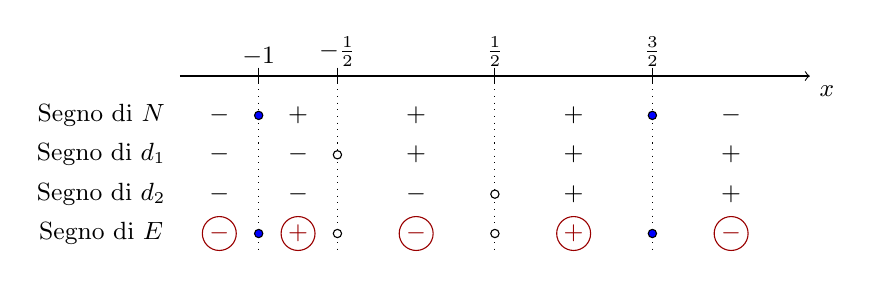
\begin{tikzpicture}[font=\small,x=10mm, y=10mm]

\draw[->] (0,0) -- (8,0) node [below right] () {$x$};

\foreach \x in {1,2,4,6}{
\draw(\x,3pt)--(\x,-3pt);
\begin{scope}[dotted]
\draw (\x,0) -- (\x,-2.2);
\end{scope}}
\node[] at (-1,-0.5) {Segno di $N$};
\draw[fill=blue] (1,-.5)circle (1.5pt);
\draw[fill=blue] (6,-.5)circle (1.5pt);
\node[] at (-1,-1) {Segno di $d_1$};
\draw[fill=white] (2,-1)circle (1.5pt);
\node[] at (-1,-1.5) {Segno di $d_2$};
\draw[fill=white] (4,-1.5)circle (1.5pt);
\node[] at (-1,-2) {Segno di $E$};
\draw[fill=blue] (1,-2)circle (1.5pt);
\draw[fill=blue] (6,-2)circle (1.5pt);
\draw[fill=white] (2,-2)circle (1.5pt);
\draw[fill=white] (4,-2)circle (1.5pt);
\node[above]  at (1,0) {$-1$};
\node[above]  at (2,0) {$-{\frac{1}{2}}$};
\node[above]  at (4,0) {${\frac{1}{2}}$};
\node[above]  at (6,0) {${\frac{3}{2}}$};
\node[] at (.5,-0.5) {$-$};
\node[] at (1.5,-0.5) {$+$};
\node[] at (3,-0.5) {$+$};
\node[] at (5,-0.5) {$+$};
\node[] at (7,-0.5) {$-$};
\node[] at (.5,-1) {$-$};
\node[] at (1.5,-1) {$-$};
\node[] at (3,-1) {$+$};
\node[] at (5,-1) {$+$};
\node[] at (7,-1) {$+$};
\node[] at (.5,-1.5) {$-$};
\node[] at (1.5,-1.5) {$-$};
\node[] at (3,-1.5) {$-$};
\node[] at (5,-1.5) {$+$};
\node[] at (7,-1.5) {$+$};

\begin{scope}[red!60!black]
\node[circle,inner sep=1pt,draw] at (.5,-2) {$-$};
\node[circle,inner sep=1pt,draw] at (1.5,-2) {$+$};
\node[circle,inner sep=1pt,draw] at (3,-2) {$-$};
\node[circle,inner sep=1pt,draw] at (5,-2) {$+$};
\node[circle,inner sep=1pt,draw] at (7,-2) {$-$};
\end{scope}

\end{tikzpicture}

\end{center}
\item dalla tabella dei segni possiamo ottenere la risposta al problema posto:
\begin{itemize*}
\item l'espressione $E$ si annulla per $x=-1\vee x=\frac 3 2$;
\item l'espressione $E$ è positiva per $x\in A=\left\{x\in \insR \mid -1<x<-\frac 1 2\vee \frac 1 2<x<\frac 3 2\right\}$;
\item l'espressione $E$ è negativa per $x\in B=\left\{x\in \insR \mid x<-1\vee -\frac 1 2<x<\frac 1 2\vee x>\frac 3 2\right\}$.
\end{itemize*}
\end{enumeratea}
\end{esempio}

\begin{esempio}
Determiniamo l'insieme soluzione della disequazione: $3-\dfrac 1{2x+1}\ge \dfrac 1{1-x}$.
\begin{enumeratea}
\item Trasportiamo al primo membro la frazione del secondo membro $E=3-\frac 1{2x+1}-\frac 1{1-x}$ ed eseguiamo i calcoli ottenendo: $E=\frac{-6x^2+2x+1}{(2x+1)\cdot (1-x)}$;
\item determiniamo il dominio: $\CE\; 2x+1\neq 0\;\wedge\; 1-x\neq 0 \:\Rightarrow\: \Dom=\insR-\left\{-\frac 1 2\text{, }1\right\}$;
\item impostiamo la disequazione: $\frac{-6x^2+2x+1}{(2x+1)\cdot (1-x)}\ge 0$ che ci permetterà di rispondere al quesito posto dal problema;
\item studiamo il segno del numeratore e del denominatore:
\begin{itemize*}
\item segno di $N$: $-6x^2+2x+1\ge 0$ disequazione di secondo grado, quindi scritta l'equazione associata $-6x^2+2x+1=0$, calcoliamone il discriminante: $\frac{\Delta } 4=7$, positivo per cui si hanno due soluzioni $x_{1\text{,}2}=\frac{1\pm \sqrt 7} 6$; essendo il primo coefficiente negativo si ha $N\ge 0$ per $\frac{1-\sqrt 7} 6\le x\le \frac{1+\sqrt 7} 6$;
\item segno di $D$: $-2x^2+x+1>0$ disequazione di secondo grado; il denominatore ha due zeri reali $x=-\frac 1 2$ e $x_2=1$, il primo coefficiente è negativo, pertanto $D>0$ per $-\frac 1 2<x<1$ che rispetta le $\CE$: $x_1\neq -\frac 1 2\;\wedge\; x_2\neq 1$;
\end{itemize*}
\item compiliamo la tabella dei segni:
\begin{center}
 % (c) 2013 Claudio Carboncini - claudio.carboncini@gmail.com
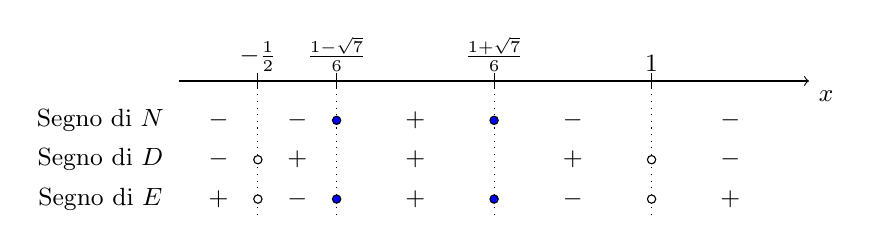
\begin{tikzpicture}[font=\small,x=10mm, y=10mm]

\draw[->] (0,0) -- (8,0) node [below right] () {$x$};

\foreach \x in {1,2,4,6}{
\draw(\x,3pt)--(\x,-3pt);
\begin{scope}[dotted]
\draw (\x,0) -- (\x,-1.7);
\end{scope}}

\node[] at (-1,-0.5) {Segno di $N$};
\draw[fill=blue] (2,-.5)circle (1.5pt);
\draw[fill=blue] (4,-.5)circle (1.5pt);
\node[] at (-1,-1) {Segno di $D$};
\draw[fill=white] (1,-1)circle (1.5pt);
\draw[fill=white] (6,-1)circle (1.5pt);
\node[] at (-1,-1.5) {Segno di $E$};
\draw[fill=blue] (2,-1.5)circle (1.5pt);
\draw[fill=blue] (4,-1.5)circle (1.5pt);
\draw[fill=white] (1,-1.5)circle (1.5pt);
\draw[fill=white] (6,-1.5)circle (1.5pt);
\node[above]  at (1,0) {$-{\frac{1}{2}}$};
\node[above]  at (2,0) {${\frac{1-\sqrt{7}}{6}}$};
\node[above]  at (4,0) {${\frac{1+\sqrt{7}}{6}}$};
\node[above]  at (6,0) {$1$};
\node[] at (.5,-0.5) {$-$};
\node[] at (1.5,-0.5) {$-$};
\node[] at (3,-0.5) {$+$};
\node[] at (5,-0.5) {$-$};
\node[] at (7,-0.5) {$-$};
\node[] at (.5,-1) {$-$};
\node[] at (1.5,-1) {$+$};
\node[] at (3,-1) {$+$};
\node[] at (5,-1) {$+$};
\node[] at (7,-1) {$-$};
\node[] at (.5,-1.5) {$+$};
\node[] at (1.5,-1.5) {$-$};
\node[] at (3,-1.5) {$+$};
\node[] at (5,-1.5) {$-$};
\node[] at (7,-1.5) {$+$};

\end{tikzpicture}

\end{center}
\item determiniamo $\IS=\left\{x\in \insR \mid x<-\frac 1 2\vee \frac{1-\sqrt 7} 6\le x\le \frac{1+\sqrt 7} 6\vee x>1\right\}$.
\end{enumeratea}
\end{esempio}
\end{exrig}

\vspazio\ovalbox{\risolvii \ref{ese:4.51}, \ref{ese:4.52}, \ref{ese:4.53}, \ref{ese:4.54}, \ref{ese:4.55}, \ref{ese:4.56}, \ref{ese:4.57}, \ref{ese:4.58}, \ref{ese:4.59}, \ref{ese:4.60}, \ref{ese:4.61}, \ref{ese:4.62}, \ref {ese:4.63},}

\vspazio\ovalbox{\ref{ese:4.64}, \ref{ese:4.65}, \ref{ese:4.66}, \ref{ese:4.67}, \ref{ese:4.68}, \ref{ese:4.69}, \ref{ese:4.70}}

\section{Sistemi di disequazioni}

Ricordiamo che risolvere un sistema di disequazioni significa trovare l'insieme dei numeri reali che sono le soluzioni comuni alle disequazioni che lo compongono. Indicate con $d_{1}$, $d_{2}$, \ldots, $d_n$ le disequazioni che formano il sistema e $\IS_{1}$, $\IS_{2}$, \ldots, $\IS_n$ i rispettivi insieme soluzione, la soluzione del sistema, indicata con $\IS$, è data da $\IS=\IS_1\cap \IS_{2}\cap \ldots \cap \IS_n$.

\begin{problema}
Nell'equazione $x^2-(k-3)x+k^2-3k+1=0$, determinare per quali valori del parametro $k$ si ottengono soluzioni reali e concordi.
\end{problema}
Abbiamo già affrontato un problema di questo tipo discutendo le equazioni parametriche di secondo grado e dunque sappiamo che la richiesta del problema esige che il discriminante ($\Delta$) sia non negativo affinché le soluzioni siano reali e che il prodotto delle stesse sia positivo. Pertanto il problema è formalizzato con un sistema di disequazioni: $\left\{\begin{array}{l}{\Delta \ge 0}\\{\frac c a>0}\end{array}\right. \Rightarrow \left\{\begin{array}{l}{k^2-6k+9-4k^2+12k-4\ge 0}\\{k^2-3k+1>0}\end{array}\right.$.

Risolviamo separatamente le due disequazioni del sistema; indicati con $\IS_1$ e $\IS_2$ rispettivamente gli insiemi soluzione della prima e della seconda disequazione, l'insieme soluzione del sistema è dato da $\IS=\IS_1\cap \IS_2$ (insieme intersezione degli insiemi soluzione delle due disequazioni).
\begin{itemize*}
\item $d_1$: $-3k^2+6k+5\ge 0$ disequazione di secondo grado avente primo coefficiente negativo e $\frac{\Delta} 4=24>0$; la parabola $y=-3k^2+6k+5\ge 0$ ha concavità verso il basso e discriminante positivo, per cui essendo $x_1=\frac{3-2\sqrt 6} 3\vee x_2=\frac{3+2\sqrt 6} 3$ si ottiene $\IS_1=\left\{x\in \insR \mid \frac{3-2\sqrt 6} 3\le x\le \frac{3+2\sqrt 6} 3\right\}$.
\item $d_2$: $k^2-3k+1>0$ disequazione di secondo grado avente il primo coefficiente positivo e $\Delta =5>0$; la parabola $y=k^2-3k+1>0$ ha concavità verso l'alto e discriminante positivo, quindi $x_1=\frac{3-\sqrt 5} 2\vee x_2=\frac{3+\sqrt 5} 2 \:\Rightarrow\: \IS_2=\left\{x\in \insR \mid x<\frac{3-\sqrt 5} 2\vee x>\frac{3+\sqrt 5} 2\right\}$.
\end{itemize*}
Per determinare l'insieme soluzione del sistema rappresentiamo in un grafico gli insiemi soluzioni delle disequazioni risolte e visualizziamo l'insieme formato dai valori che appartengono contemporaneamente ai due: sull'asse reale depositiamo i valori numerici trovati e rappresentiamo su righe distinte i due insiemi soluzione: gli intervalli in cui cadono soluzioni della prima e della seconda disequazione rappresentano l'insieme soluzione del sistema.
\begin{center}
 % (c) 2013 Claudio Carboncini - claudio.carboncini@gmail.com
\begin{tikzpicture}[font=\small,x=10mm, y=10mm]

\draw[->] (0,0) -- (8,0) node [below right] () {$r$};

\foreach \x in {2,3.5,5,6.5}{
\draw(\x,3pt)--(\x,-3pt);
\begin{scope}[dotted]
\draw (\x,0) -- (\x,-2);
\draw (0,-.5) -- (2,-.5);
\draw (6.5,-.5) -- (8,-.5);
\draw (3.5,-1) -- (5,-1);
\draw (0,-1.5) -- (2,-1.5);
\draw (3.5,-1.5) -- (5,-1.5);
\draw (6.5,-1.5) -- (8,-1.5);
\end{scope}}

\node[above]  at (2,0) {$\frac{3-2 \sqrt{6}}{3}$};
\node[above]  at (3.5,0) {$\frac{3- \sqrt{5}}{2}$};
\node[above]  at (5,0) {$\frac{3+ \sqrt{5}}{2}$};
\node[above]  at (6.5,0) {$\frac{3+2 \sqrt{6}}{3}$};
\pattern[pattern= north east lines, pattern color=red] (2,-2) rectangle (3.5,-1.5);
\pattern[pattern= north east lines, pattern color=red] (5,-2) rectangle (6.5,-1.5);

\node[] () at (-.5,-.5) {$\IS_{1}$};
\node[] () at (-.5,-1) {$\IS_{2}$};
\node[] () at (-.5,-1.75) {$\IS$};

\begin{scope}[blue,thick]
\draw (2,-.5) -- (6.5,-.5);
\draw (0,-1) -- (3.5,-1);
\draw (5,-1) -- (8,-1);
\draw (2,-1.5) -- (3.5,-1.5);
\draw (5,-1.5) -- (6.5,-1.5);

\draw[fill=blue] (2,-.5)circle (1.5pt);
\draw[fill=blue] (6.5,-.5)circle (1.5pt);
\draw[fill=white] (3.5,-1)circle (1.5pt);
\draw[fill=white] (5,-1)circle (1.5pt);
\draw[fill=blue] (2,-1.5)circle (1.5pt);
\draw[fill=blue] (6.5,-1.5)circle (1.5pt);
\draw[fill=white] (3.5,-1.5)circle (1.5pt);
\draw[fill=white] (5,-1.5)circle (1.5pt);

\end{scope}

\end{tikzpicture}

\end{center}
 $\IS=\left\{x\in \insR\mid\frac{3-2\sqrt 6} 3\le x<\frac{3-\sqrt 5} 2\vee \frac{3+\sqrt 5} 2<x\le \frac{3+2\sqrt 6} 3\right\}$. % o, scritto utilizzando gli intervalli, $\left[\frac{3-2\sqrt 6} 3\text{, }\frac{3-\sqrt 5} 2\right)\cup \left(\frac{3+\sqrt 5} 2\text{, }\frac{3+2\sqrt 6} 3\right]$.

\pagebreak
\begin{problema}
Risolvere il seguente sistema di disequazioni: $\left\{\begin{array}{l}2x^3-9x^2+10x-3\le 0\\ \frac{x^2+x+1}{\ x^3-x}\ge 0 \\3-4x<0 \end{array}\right.$.
\end{problema}

Il sistema è formato da tre disequazioni; risolviamo separatamente ciascuna disequazione:

\begin{itemize*}
\item $d_1$: $2x^3-9x^2+10x-3\le 0$ di terzo grado, scomponiamo in fattori. $x=1$ è uno zero del polinomio quindi con la regola di Ruffini otteniamo $d_1$: $(x-1)(2x^2-7x+3)\le 0$. L'equazione di secondo grado $2x^2-7x+3=0$ ha soluzioni reali $x_1=\frac 1 2\;\vee\; x=3$. Si tratta allora di studiare il segno dei singoli fattori e di determinare il segno richiesto dopo aver costruito la tabella dei segni:
\begin{center}
 % (c) 2013 Claudio Carboncini - claudio.carboncini@gmail.com
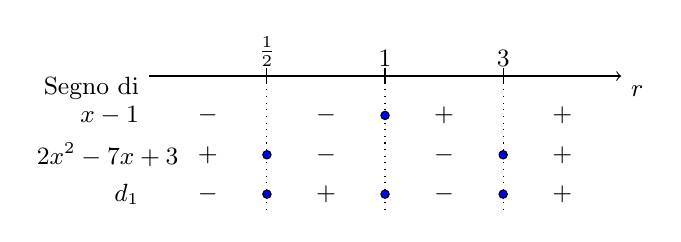
\begin{tikzpicture}[font=\small,x=10mm, y=10mm]

\draw[->] (0,0) -- (6,0) node [below right] () {$r$};

\foreach \x in {1.5,3,4.5}{
\draw(\x,3pt)--(\x,-3pt);
\begin{scope}[dotted]
\draw (\x,0) -- (\x,-1.7);
\end{scope}}

\node[left] at (0,-0.15) {Segno di};
\node[left] at (0,-0.5) {$x-1$};
\node[left] at (.5,-1) {$2x^2-7x+3$};
\node[left] at (0,-1.5) {$d_1$};
\node[above]  at (1.5,0) {$\frac{1}{2}$};
\node[above]  at (3,0) {$1$};
\node[above]  at (4.5,0) {$3$};
\node[] at (.75,-0.5) {$-$};
\node[] at (2.25,-0.5) {$-$};
\node[] at (3.75,-0.5) {$+$};
\node[] at (5.25,-0.5) {$+$};
\node[] at (.75,-1) {$+$};
\node[] at (2.25,-1) {$-$};
\node[] at (3.75,-1) {$-$};
\node[] at (5.25,-1) {$+$};
\node[] at (.75,-1.5) {$-$};
\node[] at (2.25,-1.5) {$+$};
\node[] at (3.75,-1.5) {$-$};
\node[] at (5.25,-1.5) {$+$};

\draw[fill=blue] (3,-.5)circle (1.5pt);
\draw[fill=blue] (1.5,-1)circle (1.5pt);
\draw[fill=blue] (4.5,-1)circle (1.5pt);
\draw[fill=blue] (3,-1.5)circle (1.5pt);
\draw[fill=blue] (1.5,-1.5)circle (1.5pt);
\draw[fill=blue] (4.5,-1.5)circle (1.5pt);

\end{tikzpicture}

\end{center}
L'insieme soluzione, tenendo conto che cerchiamo i valori per i quali $d_1$ risulta minore o uguale a $0$ è $\IS_1=\left\{x\in \insR \mid x\le\frac 1 2\vee 1\le x\le 3\right\}$.

\item $d_2$: $\frac{x^2+x+1}{x^3-x}\ge 0$ è una disequazione fratta, per prima cosa scomponiamo in fattori il denominatore: $\frac{x^2+x+1}{x(x^2-1)}\ge 0$.
Studiamo poi il segno dei singoli fattori o divisori, tenendo conto che $x^2+x+1=0$ ha $\Delta <0$, per cui $x^2+x+1$ è sempre positivo.
\begin{center}
 % (c) 2013 Claudio Carboncini - claudio.carboncini@gmail.com
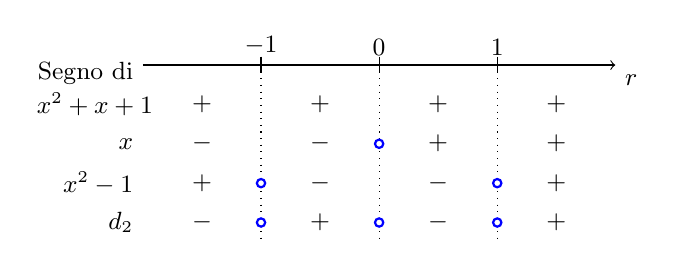
\begin{tikzpicture}[font=\small,x=10mm, y=10mm]

\draw[->] (0,0) -- (6,0) node [below right] () {$r$};

\foreach \x in {1.5,3,4.5}{
\draw(\x,3pt)--(\x,-3pt);
\begin{scope}[dotted]
\draw (\x,0) -- (\x,-2.2);
\end{scope}}

\node[left] at (0,-0.1) {Segno di};
\node[left] at (.25,-0.5) {$x^2+x+1$};
\node[left] at (0,-1) {$x$};
\node[left] at (0,-1.5) {$x^2-1$};
\node[left] at (0,-2) {$d_2$};
\node[above]  at (1.5,0) {$-1$};
\node[above]  at (3,0) {$0$};
\node[above]  at (4.5,0) {$1$};
\node[] at (.75,-0.5) {$+$};
\node[] at (2.25,-0.5) {$+$};
\node[] at (3.75,-0.5) {$+$};
\node[] at (5.25,-0.5) {$+$};
\node[] at (.75,-1) {$-$};
\node[] at (2.25,-1) {$-$};
\node[] at (3.75,-1) {$+$};
\node[] at (5.25,-1) {$+$};
\node[] at (.75,-1.5) {$+$};
\node[] at (2.25,-1.5) {$-$};
\node[] at (3.75,-1.5) {$-$};
\node[] at (5.25,-1.5) {$+$};
\node[] at (.75,-2) {$-$};
\node[] at (2.25,-2) {$+$};
\node[] at (3.75,-2) {$-$};
\node[] at (5.25,-2) {$+$};

\begin{scope}[blue,thick]
\draw[fill=white] (3,-1)circle (1.5pt);
\draw[fill=white] (1.5,-1.5)circle (1.5pt);
\draw[fill=white] (4.5,-1.5)circle (1.5pt);
\draw[fill=white] (3,-2)circle (1.5pt);
\draw[fill=white] (1.5,-2)circle (1.5pt);
\draw[fill=white] (4.5,-2)circle (1.5pt);
\end{scope}

\end{tikzpicture}

\end{center}
L'insieme soluzione, per $d_2\ge 0$ è $\IS_2=\left\{x\in \insR \mid -1<x<0\vee x>1\right\}$.
\item $d_3$: $3-4x<0$ è di primo grado per cui l'insieme soluzione è $\IS_3=\left\{x\in \insR \mid x>\frac 3 4\right\}$.
\end{itemize*}
Ricordiamo che la ricerca dell'insieme soluzione del sistema si effettua determinando l'insieme $\IS_1\cap \IS_2\cap \IS_3$ individuabile attraverso il grafico:
\begin{center}
 % (c) 2013 Claudio Carboncini - claudio.carboncini@gmail.com
\begin{tikzpicture}[font=\small,x=10mm, y=10mm]

\draw[->] (0,0) -- (8,0) node [below right] () {$r$};

\foreach \x in {1,2.3,3.4,4.5,5.6,6.7}{
\draw(\x,3pt)--(\x,-3pt);
\begin{scope}[dotted]
\draw (\x,0) -- (\x,-2.5);
\draw (3.4,-.5) -- (5.6,-.5);
\draw (6.7,-.5) -- (8,-.5);
\draw (0,-1) -- (1,-1);
\draw (2.3,-1) -- (5.6,-1);
\draw (0,-1.5) -- (4.5,-1.5);
\draw (0,-2) -- (5.6,-2);
\draw (6.7,-2) -- (8,-2);
\end{scope}}

\node[above]  at (1,0) {$-1$};
\node[above]  at (2.3,0) {$0$};
\node[above]  at (3.4,0) {$\frac{1}{2}$};
\node[above]  at (4.5,0) {$\frac{3}{4}$};
\node[above]  at (5.6,0) {$1$};
\node[above]  at (6.7,0) {$3$};
\pattern[pattern= north east lines, pattern color=red] (5.6,-2.5) rectangle (6.7,-2);

\node[] () at (-.5,-.5) {$\IS_{1}$};
\node[] () at (-.5,-1) {$\IS_{2}$};
\node[] () at (-.5,-1.5) {$\IS_{3}$};
\node[] () at (-.5,-2.25) {$\IS$};

\begin{scope}[blue,thick]
\draw (0,-.5) -- (3.4,-.5);
\draw (5.6,-.5) -- (6.7,-.5);
\draw (1,-1) -- (2.3,-1);
\draw (5.6,-1) -- (8,-1);
\draw (4.5,-1.5) -- (8,-1.5);
\draw (5.6,-2) -- (6.7,-2);

\draw[fill=blue] (3.4,-.5)circle (1.5pt);
\draw[fill=blue] (5.6,-.5)circle (1.5pt);
\draw[fill=blue] (6.7,-.5)circle (1.5pt);
\draw[fill=white] (1,-1)circle (1.5pt);
\draw[fill=white] (2.3,-1)circle (1.5pt);
\draw[fill=white] (5.6,-1)circle (1.5pt);
\draw[fill=white] (4.5,-1.5)circle (1.5pt);

\draw[fill=white] (5.6,-2)circle (1.5pt);
\draw[fill=blue] (6.7,-2)circle (1.5pt);

\end{scope}

\end{tikzpicture}

\end{center}
Il sistema è quindi verificato per $1<x\le 3$.

\vspazio\ovalbox{\risolvii \ref{ese:4.71}, \ref{ese:4.72}, \ref{ese:4.73}, \ref{ese:4.74}, \ref{ese:4.75}, \ref{ese:4.76}, \ref{ese:4.77}, \ref{ese:4.78}, \ref{ese:4.79}, \ref{ese:4.80}, \ref{ese:4.81}}
\newpage
% (c)~2014 Claudio Carboncini - claudio.carboncini@gmail.com
% (c)~2014 Dimitrios Vrettos - d.vrettos@gmail.com
\section{Esercizi}
\subsection{Esercizi dei singoli paragrafi}
\subsection*{4.1 - Risoluzione delle disequazioni di secondo grado}

\begin{esercizio}[\Ast]
 \label{ese:4.1}
Risolvi le seguenti disequazioni di secondo grado con il metodo algebrico.
\begin{multicols}{3}
 \begin{enumeratea}
 \item~$x^2-6x\le 0$;
 \item~$5x^2>0$;
 \item~$x^2+x>0$;
 \item~$x^2\le 0$;
 \item~$3x^2\le -1$;
 \item~$x^2-9>0$;
 \item~$2x^2-3x+1>0$;
 \item~$-x^2+3x\ge 0$;
 \item~$3x^2+x-2>0$;
 \item~$x^2-4>0$;
 \item~$\frac 4 3x^2-\frac 1 3x-1<0$;
 \item~$x^2-8\le 0$.
 \end{enumeratea}
 \end{multicols}
\end{esercizio}

\begin{esercizio}[\Ast]
 \label{ese:4.2}
Risolvi le seguenti disequazioni di secondo grado con il metodo algebrico.
\begin{multicols}{3}
 \begin{enumeratea}
 \item~$x^2-5x+3\ge 0$;
 \item~$x^2-4x+9>0$;
 \item~$x^2-6x+8\le 0$;
 \item~$x^2+3x-4\ge 0$;
 \item~$x^2-4x-9\le 0$;
 \item~$x^2-9x+18<0$;
 \item~$x^2-8x+15\ge 0$;
 \item~$-2x^2\ge 0$;
 \item~$3x^2-\frac 2 3x-1\le 0$;
 \item~$x^2+5>0$;
 \item~$x^2+6x-2>0$;
 \item~$2x^2+5x+4\le 0$.
 \end{enumeratea}
 \end{multicols}
\end{esercizio}

\begin{esercizio}[\Ast]
\label{ese:4.3}
Risolvi le seguenti disequazioni di secondo grado con il metodo algebrico.
\begin{multicols}{3}
 \begin{enumeratea}
 \item~$x^2-3x-\frac 5 2<0$;
 \item~$x^2+1>0$;
 \item~$-x^2+5\le 0$;
 \item~$x^2+x\ge 0$;
 \item~$(x+1)^2\ge 0$;
 \item~$x^2>1$;
 \item~$2x^2-6<0$;
 \item~$-x^2-1\le 0$;
 \item $-(x-1)^{2}\le 0$.
 \end{enumeratea}
 \end{multicols}
\end{esercizio}

\begin{esercizio}[\Ast]
\label{ese:4.4}
Risolvi le seguenti disequazioni di secondo grado con il metodo algebrico.
\begin{multicols}{3}
 \begin{enumeratea}
 \item~$x^2+1<1$;
 \item~$x^2-8x+16>0$;
 \item~$\frac{x^{2}}{2}+4x+8>0$;
 \item~$\frac{x^{2}}{3}-x-\frac{4}{3}<0$;
 \item~$x^2-8x+15<0$;
 \item~$2x^2-3x-2>0$.
 \end{enumeratea}
 \end{multicols}
\end{esercizio}

\begin{esercizio}[\Ast]
\label{ese:4.5}
Risolvi le seguenti disequazioni di secondo grado con il metodo algebrico.
\begin{multicols}{3}
 \begin{enumeratea}
 \item~$-3x^2+x+\frac 1 4<0$;
 \item~$3x^2-2x-1>0$;
 \item~$\frac{x^{2}}{5}-2x+5<0$;
 \item~$x^2+3x+8>0$;
 \item~$x^2-2x\ge 0$;
 \item~$-5x^2+4x+1\le 0$.
 \end{enumeratea}
 \end{multicols}
\end{esercizio}

\subsection*{4.2 - Risoluzione grafica di una disequazione di secondo grado}

\begin{esercizio}
 \label{ese:4.6}
Rappresentare nel riferimento cartesiano ortogonale le seguenti parabole.
\begin{multicols}{2}
 \begin{enumeratea}
 \item~$ y=-3x^2+x $;
 \item~$ y=\frac 1 2x-2x+\frac 3 2 $;
 \item~$ y=x^2+x-1 $;
 \item~$ y=x^2-x+1 $.
 \end{enumeratea}
 \end{multicols}
\end{esercizio}

\begin{esercizio}
 \label{ese:4.7}
Rappresentare nel riferimento cartesiano ortogonale le seguenti parabole.
\begin{multicols}{2}
 \begin{enumeratea}
 \item~$ y=-3x^2+3 $;
 \item~$ y=x^2+4x+3 $;
 \item~$ y=x^2+\frac 3 5 $;
 \item~$ y=-\frac 2 5x^2+4x-\frac 1 5 $.
% \item~$ y=-\frac 1 2 x^2-4x-1 $.
 \end{enumeratea}
 \end{multicols}
\end{esercizio}

\begin{esercizio}
 \label{ese:4.8}
Per ciascun grafico di parabola $y=ax^2+bx+c$ indica il segno del primo coefficiente e del discriminante, la natura dei suoi zeri (reali distinti, reali coincidenti, non reali), il segno della funzione.
\begin{center}
 % (c) 2012 Dimitrios Vrettos - d.vrettos@gmail.com
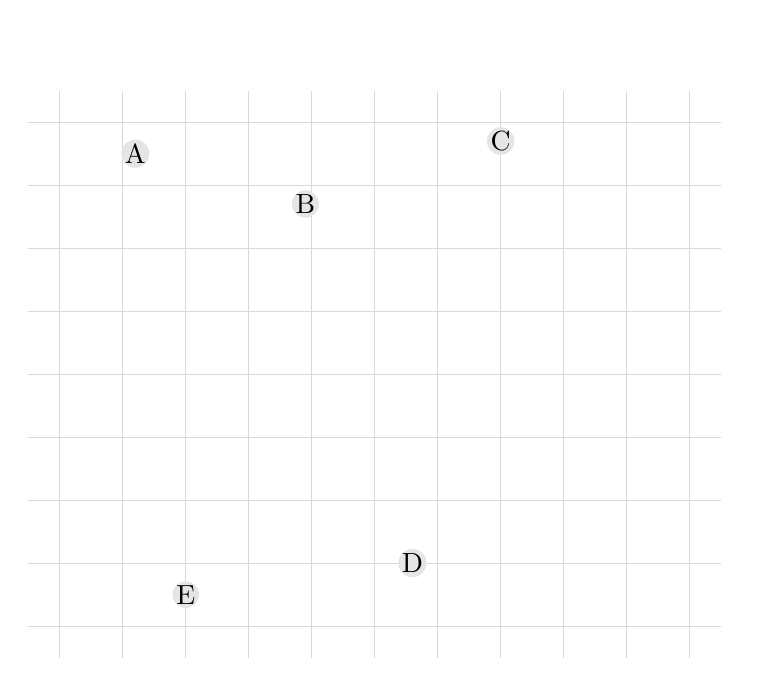
\begin{tikzpicture}[x=8mm, y=8mm]
\draw[step=0.8cm,color=gray!30] (-5.5,-4.5) grid (5.5,4.5);
  \tkzInit[xmin=-5,xmax=5,ymin=-4.5,ymax=4.5]
  \clip (-5.5,-4.5) rectangle (6,5.5);
  \begin{scope}[font=\small]
    \tkzAxeY[orig = false, label options={left = 1pt}]
    \tkzAxeX[orig = true, label options={below = 1pt}]
  \end{scope}
  \tkzFct[domain=-1.5:1.5,thick,color=darkgray]{2*x*x-1}
  \node [inner sep=0pt, circle, fill=gray!20] (a) at (-1.1, 2.7) {B};
  \tkzFct[domain=0:3,thick,color=blue]{-2*x*x+6*x-4};
  \node [inner sep=0pt, circle, fill=gray!20] (a) at (.6, -3) {D};
  \tkzFct[domain=-3.3:-.7,thick,color=RedOrange]{-2*x*x-8*x-8.5};
  \node [inner sep=0pt, circle, fill=gray!20] (a) at (-3, -3.5) {E};
  \tkzFct[domain=1.5:4.5,thick,color=purple]{2*x*x-12*x+18};
  \node [inner sep=0pt, circle, fill=gray!20] (a) at (2, 3.7) {C};
  \tkzFct[domain=-4.5:-1.5,thick,color=olive]{2*x*x+12*x+19};
  \node [inner sep=0pt, circle, fill=gray!20] (a) at (-3.8, 3.5) {A};

\end{tikzpicture}

\end{center}
\end{esercizio}

\begin{esercizio}
 \label{ese:4.9}
Risolvere graficamente le seguenti disequazioni di secondo grado.
\begin{multicols}{3}
 \begin{enumeratea}
 \item~$ 2x^2+3x-1<0 $;
 \item~$ x^2-5x+6\le 0 $;
 \item~$ x^2-3x-4>0 $;
 \item~$ x^2-6x+5\ge 0 $;
 \item~$ 6x^2+x-2>0 $;
 \item~$ 15x^2+x-6\le 0 $;
 \item~$ -x^2+1\ge 0 $;
 \item~$ x^2-\frac 1 4>0 $;
 \item~$ x^2-\frac 1 4x\le 0 $;
 \item~$ x^2+2x\le 0 $;
 \item~$ x^2+2x+1\le 0 $;
 \item~$ x^2+x+1<0 $.
 \end{enumeratea}
 \end{multicols}
\end{esercizio}

\begin{esercizio}[\Ast]
 \label{ese:4.10}
Risolvi le disequazioni di secondo grado con il metodo algebrico o con quello grafico.
\begin{multicols}{3}
 \begin{enumeratea}
 \item~$9-4x^2\le 0$;
 \item~$3x-2x^2>0$;
 \item~ $x^2\ge 0$;
 \item~$2x^2+4>0$;
 \item~$x^2-x-2>0$;
 \item~$x^2+11x+30\le 0$;
 \item~$-x^2+4x+3>0$;
 \item~$x^2+4x+4<0$;
 \item~$x^2-x+1<0$;
 \item~$x^2-\frac 1 9\ge 0$;
 \item~$9x^2+3x-2\le 0$;
 \item~$2x^2+5<0$.
 \end{enumeratea}
 \end{multicols}
\end{esercizio}

\begin{esercizio}[\Ast]
 \label{ese:4.11}
Risolvi le disequazioni di secondo grado.
\begin{multicols}{3}
 \begin{enumeratea}
 \item~$4x-x^2\ge 0$;
 \item~$9x^2+10x+1\le 0$;
 \item~$\np{0,01}x^2-1>0$;
 \item~$\np{1,}\overline{6}x^2-2x\le 0$;
 \item~$\frac 1 2x^2-\frac 1 8>0$;
 \item~$4x^2+\frac 5 3x-1\le 0$;
 \item~$x^2+x+\sqrt 2>0$;
 \item~$x^2+2\sqrt 2x+2>0$.
 \end{enumeratea}
 \end{multicols}
\end{esercizio}
\pagebreak
\begin{esercizio}[\Ast]
 \label{ese:4.12}
Risolvi le disequazioni di secondo grado.
\begin{multicols}{2}
 \begin{enumeratea}
 \item~$12x^2-3\ge 4x(2x-1)$;
 \item~$2x^2-11x-6\ge 0$;
 \item~$(3x+1)^2>(2x-1)^2$;
 \item~$(x+1)(x-1)^2>x^3$;
 \item~$(x+3)(x+2)<-(x+2)^2$;
 \item~$\frac{x+1} 2+\frac{(x+1)(x-1)} 4>x^2-1$;
 \item~$(x+1)^3-(x+2)^2>\frac{2x^3-1} 2$;
 \item~$(x-2)(3-2x)\ge x-2$.
 \end{enumeratea}
 \end{multicols}
\end{esercizio}

\begin{esercizio}[\Ast]
 \label{ese:4.13}
Risolvi le disequazioni di secondo grado.
\begin{multicols}{2}
 \begin{enumeratea}
 \item~$(3x+1)\left(\frac 5 2+x\right)\le 2x-1$;
 \item~$\frac{x^2+16} 4+x-1<\frac{x-3} 2$;
 \item~$\frac{3x-2} 2<x^2-2$;
 \item~$\frac{x-3} 2-\frac{x^2+2} 3<1+x$.
 \end{enumeratea}
 \end{multicols}
\end{esercizio}

\begin{esercizio}[\Ast]
 \label{ese:4.14}
Risolvi le disequazioni di secondo grado.
\begin{multicols}{2}
 \begin{enumeratea}
 \item~$(2x+1)^{2}>9x^{2}+24x+22$;
 \item~$(2x-1)^{2}<x^{2}+16$;
 \item~$4x(x-5)>(x-4)^{2}+47$;
 \item~$(x-2)(x+2)>3x^{2}-32+10x$.
 \end{enumeratea}
 \end{multicols}
\end{esercizio}

\begin{esercizio}[\Ast]
\label{ese:4.15}
Risolvi le disequazioni di secondo grado.
 \begin{enumeratea}
 \item~$(x+4)^2+8\ge \frac{x-1} 3$;
 \item~$\left(\frac{x-1} 3-\frac x 6\right)^2\le (x+1)^2$;
 \item~$\frac 1 2\left(x-\frac 2 3\right)^2+x\left(x-\frac 2 3\right)\left(x+\frac 2 3\right)>x^3-\frac x 2\left(x-\frac 2 3\right)-\frac 8{27}$;
 \item~$3x-5+(1-3x)^2>(x-2)(x+2)$.
 \end{enumeratea}
\end{esercizio}

\begin{esercizio}[\Ast]
 \label{ese:4.16}
Risolvi le disequazioni di secondo grado.
\begin{multicols}{2}
 \begin{enumeratea}
 \item~$\frac{3x+1}{2}\cdot\frac{3x-1}{2}<\frac{35}{4}+(2-x)^{2}$;
 \item~$\frac{2}{3}x(3-x)-(x-1)<-2\left(\frac{1}{3}+x\right)$;
 \item~$(x+2)^{2}+5>(1-x)(2x+5)$;
 \item~$3(x-2)^{2}-1>\frac{3}{2}\left(x^{2}+2\right)-x^{2}$.
 \end{enumeratea}
 \end{multicols}
\end{esercizio}

\begin{esercizio}[\Ast]
\label{ese:4.17}
Risolvi le disequazioni di secondo grado.
 \begin{enumeratea}
 \item~$\frac{x-2} 3-(3x+3)^2>x$;
 \item~$(x-4)^2+(2-x)^2-2(2x+17)>4(x+5)(3-x)+(x+1)^2$;
 \item~$(x-2)^3-x^3>x^2-4$;
 \item~$(2-x)^3-(2-x)^2<\frac{3-4x^3} 4$;
 \item~$(x+\np{2000})^2+x+\np{2000}<2$.
 \end{enumeratea}
\end{esercizio}

\begin{esercizio}[\Ast]
\label{ese:4.18}
Risolvi le disequazioni di secondo grado.
 \begin{enumeratea}
 \item~$2x^{2}+\frac{3}{2}(x-3)(5-x)<(x-3)(x-2)+\frac{x-3}{2}(17-5x)$;
 \item~$\frac{3}{4}(x-2)(4-x)+7-(5-x)^{2}>(3-x)[3(x-4)-2(x-2)]$;
 \item~$\frac{1}{3}(4x-1)^{2}-11+\frac{2}{3}(2x+1)^{2}>2(2x+1)^{2}-\frac{5}{3}(2x+3)^{2}$;
 \item~$\frac{4}{3}(x-1)+\frac{1}{9}(x-5)(5-x)+\frac{1}{6}(5x+1)^{2}>1+\frac{5}{6}(3x-1)^{2}-\frac{4}{3}(x-1)^{2}$.
 \end{enumeratea}
\end{esercizio}

\begin{esercizio}[\Ast]
 \label{ese:4.19}
Risolvi le disequazioni di secondo grado con il metodo algebrico o con quello grafico.
 \begin{enumeratea}
 \item~$\frac{\left(2x-1\right)^3-8x} 2-\frac{\left(2x+1\right)^2-15} 4\le 4x\left(x-1\right)^2-6$;
 \item~$\frac{(3-x)^2} 2-1\ge -\frac{x^2-4} 4$;
 \item~$\left(\frac x 2+1\right)^2-2x>\frac 5 4\left(\frac x 2-1\right)$;
 \item~$(x+1)^2>(x-1)^2+(x+2)^2+4x$;
 \item~$\frac{x^2} 4+x<\frac{x+3} 4+\frac x 2-\frac{1-\frac x 2} 2$.
 \end{enumeratea}
\end{esercizio}

\begin{esercizio}
\label{ese:4.20}
Il monomio $16x^2$ risulta positivo per:

\boxA\quad $x>16$\qquad \boxB\quad $x>\frac 1{16}$\qquad\boxC\quad $x\in \insR$\qquad\boxD\quad $x\in \insR_0$\qquad\boxE\quad $x<-4\vee x>16$

\end{esercizio}

\begin{esercizio}
\label{ese:4.21}
Il binomio $16+x^2$ risulta positivo per:

\boxA\; $x>-16$\quad \boxB\; $-4<x<4$ \quad\boxC\; $x\in \insR-\{-4$, $4\}$ \quad\boxD\; $x\in \insR$ \quad\boxE\; $x<-4\vee x>4$
\end{esercizio}

\begin{esercizio}
\label{ese:4.22}
Il binomio $16-x^2$ risulta positivo per:

\boxA\; $x>-16$\quad \boxB\; $-4<x<4$ \quad\boxC\; $x\in \insR-\{-4$, $4\}$ \quad\boxD\; $x\in \insR$ \quad\boxE\; $x<-4\vee x>4$
\end{esercizio}

\begin{esercizio}
 \label{ese:4.23}
Spiegate sfruttando il metodo grafico la verità della proposizione: ``nessun valore della variabile $a$ rende il polinomio $(3+a)^2-(2a+1)\cdot (2a-1)-(a^2+2a+35)$ positivo''.
\end{esercizio}

\subsection*{4.3 - Segno del trinomio a coefficienti letterali}

\begin{esercizio}[\Ast]
 \label{ese:4.24}
Risolvi e discuti le seguenti disequazioni.
\begin{multicols}{2}
 \begin{enumeratea}
 \item~$x^2-2{kx}+k^2-1>0$;
 \item~$3x^2-5{ax}-2a^2<0$;
 \item~$4x^2-4x+1-9m^2<0$;
 \item~$2x^2-3{ax}<0$.
 \end{enumeratea}
 \end{multicols}
\end{esercizio}

\begin{esercizio}[\Ast]
 \label{ese:4.25}
Risolvi e discuti le seguenti disequazioni.
\begin{multicols}{2}
 \begin{enumeratea}
 \item~$x^2-2{tx}-8t^2>0$;
 \item~$(1-s)x^2+9>0$;
 \item~$(m-1)x^2-{mx}>0$;
 \item~${kx}^2-(k+1)x-3\ge 0$.
 \end{enumeratea}
 \end{multicols}
\end{esercizio}

\begin{esercizio}
 \label{ese:4.26}
Trovare il segno del trinomio $t=(1-m)x^2-2{mx}-m+3$ al variare del parametro~$m$.
\end{esercizio}

\subsection*{4.4 - Disequazioni polinomiali di grado superiore al secondo}

\begin{esercizio}
 \label{ese:4.27}
Data la disequazione $\left(x^2-x\right)\cdot \left(2x^2+13x+20\right)<0$ verificare che nessun numero \emph{naturale} appartiene all'insieme soluzione.
\end{esercizio}

\begin{esercizio}
 \label{ese:4.28}
Dopo aver scomposto in fattori il polinomio $p(x)=2x^4-5x^3+5x-2$ determinare il suo segno.
\end{esercizio}

\begin{esercizio}
 \label{ese:4.29}
Dato il trinomio $p(x)=9x^2+x^4-10$ stabilire se esiste almeno un numero naturale che lo renda negativo.
\end{esercizio}

\begin{esercizio}
\label{ese:4.30}
Nell'insieme dei valori reali che rendono positivo il trinomio $p(x)=2x^5-12x^3-14x$ vi sono solo due numeri interi negativi?
\end{esercizio}

\begin{esercizio}
 \label{ese:4.31}
$x\in (-1;+\infty )\Rightarrow p(x)=x^5-2x^2-x+2>0$. Vero o falso?
\end{esercizio}

\begin{esercizio}
\label{ese:4.32}
Nell'insieme dei valori reali che rendono negativo $p(x)=(2x-1)^3-(3-6x)^2$ appartiene un valore razionale che lo annulla. Vero o falso?
\end{esercizio}
%\newpage
\pagebreak
\begin{esercizio}[\Ast]
\label{ese:4.33}
Risolvi le seguenti disequazioni di grado superiore al secondo.
\begin{multicols}{2}
\begin{enumeratea}
\item $(1-x)(2-x)(3-x)>0$;
\item $(2x-1)(3x-2)(4x-3)\le 0$;
\item $-2x(x-1)(x+2)>0$;
\item $ \left(x^2-4x-45\right)\cdot \left(4x^2-4x+1\right)>0 $;
\item $3x(x-2)(x+3)(2x-1)\le 0$;
\item $\left(x^2+1\right)(x-1)(x+2)>0$;
\item $\left(1-9x^2\right)\left(9x^2-3x\right)2x>0$;
\item $\left(16x^2-1\right)\left(x^2-x-12\right)>0$.
\end{enumeratea}
\end{multicols}
\end{esercizio}

\begin{esercizio}[\Ast]
\label{ese:4.34}
Risolvi le seguenti disequazioni di grado superiore al secondo.
\begin{multicols}{2}
\begin{enumeratea}
\item $-x\left(x^2-3x-10\right)\left(x^2-9x+18\right)\le 0$;
\item $x^2(x-1)\left(2x^2-x\right)\left(x^2-3x+3\right)>0$;
\item $\left(x^2-1\right)\left(x^2-2\right)\left(x^2-3x\right)>0$;
\item $x^3-x^2+x-1>0$;
\item $x^3-5x^2+6<0$;
\item $\left(5x^3-2x^2\right)\left(3x^2-5x\right)\ge 0$;
\item $x^4-2x^3-x+2>0$;
\item $x^4+x^2-9x^2-9\le 0$.
\end{enumeratea}
\end{multicols}
\end{esercizio}

\begin{esercizio}[\Ast]
\label{ese:4.35}
Risolvi le seguenti disequazioni di grado superiore al secondo.
\begin{multicols}{2}
\begin{enumeratea}
\item $25x^4-9>0$;
\item $x^3-1\ge 2x(x-1)$;
\item $x^4-1>x^2+1$;
\item $\left(x^2+x\right)^2+2\left(x+1\right)^2\ge 0$;
\item $(x+1)\left(x-\frac 1 2\right)(x+2)<0$;
\item $\left(x^2-4\right)(x-2)\ge 0$; %~~~~R.~~$x\ge -2$;
\item $(x-7)\left(x^2-7x+10\right)<0$;
\item $\left(x^2-4\right)\left(x^2-9\right)\ge 0$.
\end{enumeratea}
\end{multicols}
\end{esercizio}

\begin{esercizio}[\Ast]
 \label{ese:4.36}
Risolvi le seguenti disequazioni di grado superiore al secondo.
\begin{multicols}{2}
\begin{enumeratea}
\item $\left(x^4+4x^3-12x^2\right)\left(x+3\right)\ge 0$;
\item $(x-4)^3-(x-4)^2-2x+10>2$;
\item $x^3-1\ge 0$;
\item $\left(x^4+4x^3-12x^2\right)\left(x+3\right)\ge 0$.
\end{enumeratea}
\end{multicols}
\end{esercizio}

\begin{esercizio}[\Ast]
 \label{ese:4.37}
Risolvi le seguenti disequazioni di grado superiore al secondo.
\begin{multicols}{2}
\begin{enumeratea}
\item $(x+4)(x+5)(5-x)(4-x)>0$;
\item $(x^2-2x)(x^2+1)>0$;
\item $(8-2x^2)(3x-x^2+4)<0$;
\item $(6x^2-6)(100x^2+100x)<0$.
\end{enumeratea}
\end{multicols}
\end{esercizio}

\begin{esercizio}[\Ast]
 \label{ese:4.38}
Risolvi le seguenti disequazioni di grado superiore al secondo.
\begin{multicols}{2}
\begin{enumeratea}
\item $(1+x^2)(3x^2+x)<0$;
\item $(x^2+3x+3)(4x^2+3)>0$;
\item $(125+4x^2)(128+2x^2)<0$;
\item $(x^2+4x+4)(x^2-4x+3)>0$.
\end{enumeratea}
\end{multicols}
\end{esercizio}

\begin{esercizio}[\Ast]
 \label{ese:4.39}
Risolvi le seguenti disequazioni di grado superiore al secondo.
\begin{multicols}{2}
\begin{enumeratea}
\item $(x^2-5x+8)(x^2-2x+1)>0$;
\item $(-2x+1)(3x-x^2)>0$;
\item $(4x^2-3x)(x^2-2x-8)<0$;
\item $(4x-x^2+5)(x^2-9x+20)<0$.
\end{enumeratea}
\end{multicols}
\end{esercizio}

\begin{esercizio}[\Ast]
 \label{ese:4.40}
Risolvi le seguenti disequazioni di grado superiore al secondo.
\begin{multicols}{2}
\begin{enumeratea}
\item $(5+2x)(-2x^2+14x+16)<0$;
\item $(5x-2x^2-10)(x^2+3x-28)>0$;
\item $(x^2-6x+9)(8x-7x^2)>0$;
\item $(3x^2+2x-8)(6x^2+19x+15)<0$.
\end{enumeratea}
\end{multicols}
\end{esercizio}
\pagebreak
\begin{esercizio}[\Ast]
 \label{ese:4.41}
Risolvi le seguenti disequazioni di grado superiore al secondo.
\begin{multicols}{2}
\begin{enumeratea}
\item $(3x^2-5x-2)(4x^2+8x-5)>0$;
\item $(4x-4)(2x^2-3x+2)<0$;
\item $(2x-4)(2x^2-3x-14)>0$;
\item $(-7x+6)(x^2+10x+25)<0$.
\end{enumeratea}
\end{multicols}
\end{esercizio}

\begin{esercizio}[\Ast]
 \label{ese:4.42}
Risolvi le seguenti disequazioni di grado superiore al secondo.
\begin{multicols}{2}
\begin{enumeratea}
\item $(-3+3x)(x^3-4x^2)>0$;
\item $\left(x^2+1\right)\left(x^2-1\right)>0$;
\item $(1-x)(2-x)^2\le 0$;
\item $-x\left(x^2+1\right)(x+1)\ge 0$;
\item $(x+1)^2\left(x^2-1\right)<0$;
\item $(x^2-4)(2x-50x^2)\ge 0$.
\end{enumeratea}
\end{multicols}
\end{esercizio}

\begin{esercizio}[\Ast]
 \label{ese:4.43}
Risolvi le seguenti disequazioni di grado superiore al secondo.
\begin{multicols}{2}
\begin{enumeratea}
\item $(x-4)(2x^2+x-1)\ge 0$;
\item $-3x^3+27>0$;
\item $3x^3+27>0$;
\item $x^3+3x^2+3x+1\le 0$;
\item $x^3-6x+9<0$;
\item $x^5+1>x\left(x^3+1\right)>0$.
\end{enumeratea}
\end{multicols}
\end{esercizio}

\begin{esercizio}[\Ast]
 \label{ese:4.44}
Risolvi le seguenti disequazioni di grado superiore al secondo.
\begin{multicols}{2}
\begin{enumeratea}
\item $x^3-7x^2+4x+12\ge 0$;
\item $x^3+5x^2-2x-24<0$;
\item $6x^3+23x^2+11x-12\le 0$;
\item $4x^3+4x^2-4x-4\ge 0$;
\item $-6x^3-30x^2+192x-216<0$;
\item $81x^4-1\le 0$.
\end{enumeratea}
\end{multicols}
\end{esercizio}

\begin{esercizio}[\Ast]
 \label{ese:4.45}
Risolvi le seguenti disequazioni di grado superiore al secondo.
\begin{multicols}{2}
\begin{enumeratea}
\item $3x^5+96<0$;
\item $x^4-13x^2+36<0$;
\item $9x^4-37x^2+4\ge 0$;
\item $-4x^4+65x^2-16<0$;
\item $x^6-4x^3+3\ge 0$;
\item $x^8-x^4-2<0$.
\end{enumeratea}
\end{multicols}
\end{esercizio}

\begin{esercizio}[\Ast]
 \label{ese:4.46}
Risolvi le seguenti disequazioni di grado superiore al secondo.
\begin{enumeratea}
\item $\dfrac 2 3x^3>\dfrac 9 4$;
\item $ (2x-1)^2\ge x^2\left(4x^2-4x+1\right) $;
\item $ (x-1)\left(x^2-1\right)>\left(x^2-x\right)(x-1)^2 $;
\item $ -4x\left(x^2+7x+12\right)\left(x^2-25\right)(4-x)>0 $;
\item $ (x-5x^2)(x^4-3x^3+5x^2)\ge 0 $;
\item $ (4+7x^2)\left[x^2-(\sqrt 2+\sqrt 3)x+\sqrt 6\right]<0 $.
\end{enumeratea}
\end{esercizio}
%\newpage
%\pagebreak
\begin{esercizio}[\Ast]
 \label{ese:4.47}
Risolvi le seguenti disequazioni di grado superiore al secondo.
\begin{multicols}{2}
\begin{enumeratea}
\item $ (x^3-9x)(x-x^2)(4x-4-x^2)>0 $;
\item $ x\left|x+1\right|\cdot (x^2-2x+1)\ge 0 $;
\item $16x^4-1\ge 0$;
\item $16x^4+1\le 0$;
\item $-16x^4-1>0$;
\item $-16x^4+1>0$.
\end{enumeratea}
\end{multicols}
\end{esercizio}
\pagebreak
\begin{esercizio}[\Ast]
 \label{ese:4.48}
Risolvi le seguenti disequazioni di grado superiore al secondo.
\begin{multicols}{3}
\begin{enumeratea}
\item $1-16x^4<0$;
\item $27x^3-8\ge 0$;
\item $8x^3+27<0$;
\item $4x^4+1\ge 0$;
\item $4x^4-1\ge 0$;
\item $\np{1000}x^3+27>0$.
\end{enumeratea}
\end{multicols}
\end{esercizio}

\begin{esercizio}[\Ast]
 \label{ese:4.49}
Risolvi le seguenti disequazioni di grado superiore al secondo.
\begin{multicols}{3}
\begin{enumeratea}
\item $\np{10000}x^4-1\ge 0$;
\item $x^7+7<0$;
\item $x^3-8\ge 0$;
\item $9x^4-4\ge 0$;
\item $x^6+\sqrt 6\le 0$;
\item $\np{0,1}x^4-\np{1000}\ge 0$;
\item $x^4-9\ge 0$;
\item $x^4+9\le 0$;
\item $-x^4+9\le 0$.
\end{enumeratea}
\end{multicols}
\end{esercizio}

\begin{esercizio}[\Ast]
 \label{ese:4.50}
Risolvi le seguenti disequazioni con la regola di Ruffini, dopo avere determinato per tentativi una o più radici.
\begin{multicols}{2}
\begin{enumeratea}
\item $x^{3}-3x^{2}-9x-5>0$;
\item $2x^{3}-9x^{2}+10x-3<0$;
\item $x^{3}-4x^{2}-19x-14\ge 0$;
\item $4x^{3}+8x^{2}-11x+3\le 0$;
\item $x^{4}-4x^{3}+3x^{2}+4x-4\le 0$;
\item $x^{4}+8x^{3}+22x^{2}+24x+9\ge 0$.
\end{enumeratea}
\end{multicols}
\end{esercizio}

\subsection*{4.5 - Disequazioni fratte}

\begin{esercizio}[\Ast]
 \label{ese:4.51}
Determinare l'Insieme Soluzione delle seguenti disequazioni fratte.
\begin{multicols}{3}
\begin{enumeratea}
\item $\frac{x+2}{x-1}>0$;
\item $\frac{x+3}{4-x}>0$;
\item $\frac{x+5}{x-7}>0$;
\item $\frac{2-4x}{3x+1}\ge 0$;
\item $\frac{x^2-4x+3}{4-7x}\ge 0$;
\item $\frac{x+5}{x^2-25}>0$.
\end{enumeratea}
\end{multicols}
\end{esercizio}

\begin{esercizio}[\Ast]
 \label{ese:4.52}
Determinare l'Insieme Soluzione delle seguenti disequazioni fratte.
\begin{multicols}{3}
\begin{enumeratea}
\item $\frac{x^2-1}{x-2}>0$;
\item $\frac{x^2-4x+3}{x+5}<0$;
\item $\frac{-x^2+4x-3}{x+5}>0$;
\item $\frac{x^2+1}{x^2-2x}>0$;
\item $\frac{9-x^2}{2x^2-x-15}>0$;
\item $\frac{x^2-7x}{-x^2-8}>0$.
\end{enumeratea}
\end{multicols}
\end{esercizio}

\begin{esercizio}[\Ast]
 \label{ese:4.53}
Determinare l'Insieme Soluzione delle seguenti disequazioni fratte.
\begin{multicols}{3}
\begin{enumeratea}
\item $\frac{x+2}{x-1}\le 0$;
\item $\frac 1{x^2+2x+1}>0$;
\item $\frac{-3}{-x^2-4x-8}>0$;
\item $\frac{x^2+2x+3}{-x^2-4}>0$;
\item $\frac{3x-12}{x^2-9}>0$;
\item $\frac{5-x}{x^2-4}>0$.
\end{enumeratea}
\end{multicols}
\end{esercizio}

\begin{esercizio}[\Ast]
 \label{ese:4.54}
Determinare l'Insieme Soluzione delle seguenti disequazioni fratte.
\begin{multicols}{3}
\begin{enumeratea}
\item $\frac{3x-x^2-2}{2x^2+5x+3}>0$;
\item $\frac{4-2x}{x^2-2x-8}>0$;
\item $\frac{x^2-4x+3}{5-10x}>0$;
\item $\frac{x^2+3x+10}{4-x^2}>0$;
\item $\frac{x^2-3x+2}{4x-x^2-5}>0$;
\item $\frac{x^2+2}{25-x^2}>0$.
\end{enumeratea}
\end{multicols}
\end{esercizio}

\begin{esercizio}[\Ast]
 \label{ese:4.55}
Determinare l'Insieme Soluzione delle seguenti disequazioni fratte.
\begin{multicols}{3}
\begin{enumeratea}
\item $\frac{3x^2-2x-1}{4-2x}>0$;
\item $\frac{x+2}{x^2+4x+4}>0$;
\item $\frac{x+2}{x^2+4x+2}>0$;
\item $\frac{-x^2+2x+8}{-x-1}<0$;
\item $\frac{x^2+3x+2}{25-x^2}>0$;
\item $\frac{x^2+4x+3}{3x-6}>0$.
\end{enumeratea}
\end{multicols}
\end{esercizio}
%\newpage
\pagebreak
\begin{esercizio}[\Ast]
 \label{ese:4.56}
Determinare l'Insieme Soluzione delle seguenti disequazioni fratte.
\begin{multicols}{3}
\begin{enumeratea}
\item $\frac{5-x}{x^2-4x+3}>0$;
\item $\frac{1-x^2}{x^2+2x+3}<0$;
\item $\frac{x^2-9}{x^2-5x}>0$;
\item $\frac{x^2-x-2}{x-x^2+6}>0$;
\item $\frac{x^2-5x+6}{-3x+7}<0$;
\item $\frac{2x+8}{x^2+4x-12}>0$.
\end{enumeratea}
\end{multicols}
\end{esercizio}

\begin{esercizio}[\Ast]
 \label{ese:4.57}
Determinare l'Insieme Soluzione delle seguenti disequazioni fratte.
\begin{multicols}{3}
\begin{enumeratea}
\item $\frac{x^2-2x-63}{4x+5-x^2}>0$;
\item $\frac{4-x^2+3x}{x^2-x}>0$;
\item $\frac{x^2-2x}{5-x^2}>0$;
\item $\frac{x^2-x-2}{-3x^2+3x+18}\le 0$;
\item $\frac{x^2-8x+15}{x^2+3x+2}>0$;
\item $\frac{4x+7}{3x^2-x-2}>0$.
\end{enumeratea}
\end{multicols}
\end{esercizio}
 
\begin{esercizio}[\Ast]
 \label{ese:4.58}
Determinare l'Insieme Soluzione delle seguenti disequazioni fratte.
\begin{multicols}{2}
\begin{enumeratea}
\item $\frac{-x^2-4x-3}{6x-x^2}>0$;
\item $\frac{5x+x^2+4}{6x^2-6x}>0$;
\item $\frac{9-x^2}{x^2+5x+6}\cdot \frac{6x-2x^2}{4-x^2}>0$;
\item $\frac{2x-4x^2}{x^2+x-12}\cdot \frac{16-x^2}{5x-x^2}\le 0$;
\item $\frac{1-x^2}{x^2}\le \frac 1{x^2}-x^2-\frac 1 2$;
\item $\frac{x+2}{x-1}\ge \frac{24}{x+1}-\frac x{x^2-1}$.
\end{enumeratea}
\end{multicols}
\end{esercizio}
 
\begin{esercizio}[\Ast]
 \label{ese:4.59}
Determinare l'Insieme Soluzione delle seguenti disequazioni fratte.
\begin{multicols}{2}
\begin{enumeratea}
\item $\frac{x+1}{(x+2)(x-4)}<0$;
\item $3\cdot\frac{1-x}{x+1}-8>3\cdot\frac{x+1}{1-x}$;
\item $\frac{x(x-4)(x+1)}{x-1}<0$;
\item $\frac{x^2-6x+5}{2x-1}<0$;
\item $\frac{x^2-4}{1-x}\le 0$;
\item $\frac{3x-2}{2x^2-2x+\frac{1}{2}}\ge 0$.
\end{enumeratea}
\end{multicols}
\end{esercizio}

\begin{esercizio}[\Ast]
 \label{ese:4.60}
Determinare l'Insieme Soluzione delle seguenti disequazioni fratte.
\begin{multicols}{2}
\begin{enumeratea}
\item $\frac 1 x+\frac 1{x-1}+\frac 1{x+1}<\frac{2x+1}{x^2-1}$;
\item $\frac x{x+2}\ge \frac{x-4}{x^2-4}$;
\item $\frac{4x+1}{x^2-9}+\frac{1-x}{x+3}<6-\frac x{x-3}$;
\item $\frac{x+1}{2x-1}+\frac 3{4x+10}\ge 1-\frac{2x+2}{4x^2+8x-5}$;
\item $\frac{2x+5}{(2x+4)^2}\ge \frac 2{2x+4}$;
\item $\frac{10x^2}{x^2+x-6}+\frac x{2-x}-1\le \frac 5{x+3}$.
\end{enumeratea}
\end{multicols}
\end{esercizio}

\begin{esercizio}[\Ast]
 \label{ese:4.61}
Determinare l'Insieme Soluzione delle seguenti disequazioni fratte.
\begin{multicols}{2}
\begin{enumeratea}
\item $\frac{5x+20}{5x+5}+\frac{2x-8}{2x-2}\ge 2$;
\item $\frac 8{8x^2-8x-70}-\frac 4{4x^2-4x-35}>\frac{8x+8}{4x^2-20x+21}$;
\item $\frac{4x^2-8x+19}{8x^2-36x+28}-\frac{2x-5}{4x-4}\ge \frac{8x+12}{8x-28}$;
\item $\frac{4}{3x^{2}-4x}+1<\frac {x+2}{x}+\frac{3x-2}{6x-8}$;
\item $\frac{10}{1-x^{2}}-\frac{5}{x+1}>\frac{5}{1-x}-\frac{5}{3}$;
\item $\frac{(x-1)^2}{(2-x)(x-3)}-\frac{2-x}{3-x}<\frac{x-3}{2-x}$.
\end{enumeratea}
\end{multicols}
\end{esercizio}

\begin{esercizio}[\Ast]
 \label{ese:4.62}
Determinare l'Insieme Soluzione delle seguenti disequazioni fratte.
\begin{multicols}{2}
\begin{enumeratea}
\item $\frac{12x-7}{(x+1)^{2}-7x+5}+\frac{x-2}{x-3}<\frac{1-x}{x-2}$;
\item $\frac{1+6x}{2-2x}+\frac{3}{2}>\frac{2+2x}{1-2x}$;
\item $\frac{4x^2+1}{2x(2x-2)}>\frac{1}{2x}+\frac{1}{2x-2}$;
\item $\frac{8}{x-4}<3-\frac{7}{x-1}$;
\item $2-\frac{x-2}{1+x}<\frac{4-x}{x^{2}+2x+1}$;
\item $\frac{2}{2x-1}-\frac{6}{4x^{2}-1}>\frac{2-2x}{2x+1}$.
\end{enumeratea}
\end{multicols}
\end{esercizio}
\pagebreak
\begin{esercizio}[\Ast]
 \label{ese:4.63}
Determinare l'Insieme Soluzione delle seguenti disequazioni fratte.
\begin{multicols}{2}
\begin{enumeratea}
\item $\frac{7-x}{x-6}<\frac{21-2x}{2x}-\frac{1}{2}$;
\item $\frac{8}{1-(x-1)^{2}}-\frac{x-1}{2-x}<\frac{2}{x}$;
\item $\frac{x^2-1}{x^2-9}-\frac{1}{x+3}>\frac{1-x}{x-3}$;
\item $\frac{2}{9x^{2}-15x+6}+\frac{1}{3-3x}>\frac{9x}{2-3x}$;
\item $\frac{x+1}{x+2}>\frac{2x-1}{x-1}$;
\item $\frac{1-x}{x-2}+\frac{1+2x}{1+x}>\frac{1+x}{2-x}$.
\end{enumeratea}
\end{multicols}
\end{esercizio}

\begin{esercizio}[\Ast]
 \label{ese:4.64}
Assegnate le due funzioni $f_1=\frac{x^2+1}{2x-x^2}$ e $f_2=\frac 1 x+\frac 1{x-2}$ stabilire per quali valori della variabile indipendente si ha $f_1\ge f_2$.
\end{esercizio}

\begin{esercizio}
 \label{ese:4.65}
Spiegare perché l'espressione letterale $E=\frac{1-\frac{x^2}{x^2-1}}{2+\frac{3x-1}{1-x}}$ è sempre positiva nel suo dominio.
\end{esercizio}

\begin{esercizio}[\Ast]
 \label{ese:4.66}
Per quali valori di x la funzione $y=\frac{(x-1)\cdot x-2}{5x^2-x-4}$ è maggiore o uguale a 1.
\end{esercizio}

\begin{esercizio}[\Ast]
 \label{ese:4.67}
$ x $, $ x+2 $, $ x+4 $ sono tre numeri naturali. Determinate in $ \insN $ il più piccolo numero che rende vera la proposizione: ``il doppio del primo aumentato del prodotto degli altri due è maggiore della differenza tra il doppio del terzo e il quadrato del secondo''.
\end{esercizio}

\begin{esercizio}
 \label{ese:4.68}
Date chiare e sintetiche motivazioni alla verità della seguente proposizione: “il segno della frazione $f=\frac{9-x^2+3x}{2+x^2}$ non è mai positivo e la frazione non ha zeri reali”.
\end{esercizio}

\begin{esercizio}
 \label{ese:4.69}
Stabilire se basta la condizione $x\neq 1\wedge x\neq -1$ per rendere positiva la frazione $~f=~\frac{x^3-1}{x^4-2x^2+1}$
\end{esercizio}

\begin{esercizio}
 \label{ese:4.70}
Determinare per quali valori reali la frazione $f=\frac{(x+1)^2}{4x^2-12x+9}$ risulta non superiore a 1.
\end{esercizio}

%\newpage
%\pagebreak
\subsection*{4.6 - Sistemi di disequazioni}

\begin{esercizio}[\Ast]
 \label{ese:4.71}
Risolvere i seguenti sistemi di disequazioni.
\begin{multicols}{2}
\begin{enumeratea}
\item $\left\{\begin{array}{l}x^2-4>0\\x-5\le 0\end{array}\right.$;
\item $\left\{\begin{array}{l}x^2-4x+3\le 0\\x-2x^2<-10\end{array}\right.$;
\item $\left\{\begin{array}{l}4x-x^2>0\\3x^2(x-3)>0\end{array}\right.$;
\item $\left\{\begin{array}{l}x^2+5x+6\le 0\\2x+5\le 0\end{array}\right.$.
\end{enumeratea}
\end{multicols}
\end{esercizio}

\begin{esercizio}[\Ast]
 \label{ese:4.72}
Risolvere i seguenti sistemi di disequazioni.
\begin{multicols}{2}
\begin{enumeratea}
\item $\left\{\begin{array}{l}x^2-3>0\\x-3>1\end{array}\right.$;
\item $\left\{\begin{array}{l}\frac{2x-1}{2}>\frac{x+1}{3}\\5-x<3(x-1)^{2}\end{array}\right.$;
\item $\left\{\begin{array}{l}\frac{x}{3}+\frac{1}{2}<2x-\frac{1}{3}\\(x+1)\left(\frac{1}{2}-x\right)>0\end{array}\right.$;
\item $\left\{\begin{array}{l}x^2>3x-2\\x^{2}-3x<0\end{array}\right.$.
\end{enumeratea}
\end{multicols}
\end{esercizio}

\begin{esercizio}[\Ast]
 \label{ese:4.73}
Risolvere i seguenti sistemi di disequazioni.
\begin{multicols}{2}
\begin{enumeratea}
\item $\left\{\begin{array}{l}3x-x^2-2\le 0\\x^2>49\end{array}\right.$;
\item $\left\{\begin{array}{l}3x-2>0\\x^2-1>0\\2x-x^2<0\end{array}\right.$;
\item $\left\{\begin{array}{l}x^2-4x+4\ge 0\\x<6\end{array}\right.$;
\item $\left\{\begin{array}{l}x^2-4x+4>0\\x\le 6\\1-x^2\le 0\end{array}\right.$.
\end{enumeratea}
\end{multicols}
\end{esercizio}

\begin{esercizio}[\Ast]
 \label{ese:4.74}
Risolvere i seguenti sistemi di disequazioni.
\begin{multicols}{2}
\begin{enumeratea}
\item $\left\{\begin{array}{l}(3-4x)^{2}<29-(2x-1)^{2}\\16x^{2}<8x+3\end{array}\right.$;
\item $\left\{\begin{array}{l}5x^2>13x-8\\6x^2-19x+10\ge 0\end{array}\right.$;
\item $\left\{\begin{array}{l}2x^2-2>x(x-1)\\4x^2-13x+7<-(x+3)^{2}\end{array}\right.$;
\item $\left\{\begin{array}{l}x^2<5+4x\\3x^{2}-3x>2+2x\end{array}\right.$.
\end{enumeratea}
\end{multicols}
\end{esercizio}

\begin{esercizio}[\Ast]
 \label{ese:4.75}
Risolvere i seguenti sistemi di disequazioni.
\begin{multicols}{2}
\begin{enumeratea}
\item $\left\{\begin{array}{l}x^2+6x+9<0\\x<2\\x^2+1>0\end{array}\right.$;
\item $\left\{\begin{array}{l}x^2+6x+9\le 0\\x<2\end{array}\right.$;
\item $\left\{\begin{array}{l}4x-x^2-3<0\\3x\ge 2\end{array}\right.$;
\item $\left\{\begin{array}{l}2x^2<8\\-x^2+5x>-6\\x^2(9-x^2)\le 0\end{array}\right.$.
\end{enumeratea}
\end{multicols}
\end{esercizio}

\begin{esercizio}[\Ast]
 \label{ese:4.76}
Risolvere i seguenti sistemi di disequazioni.
\begin{multicols}{2}
\begin{enumeratea}
\item $\left\{\begin{array}{l}(x^2-4x+3)(2x-4)>0\\2x-x^2\le 1\end{array}\right.$;
\item $\left\{\begin{array}{l}(3-x)(x^2-4)(x^2-2x-8)<0\\x^2-64\le 0\end{array}\right.$;
\item $\left\{\begin{array}{l}2x^2-x-1\le 0\\3x+7>0\\x^2-10x+9\le 0\end{array}\right.$;
\item $\left\{\begin{array}{l}2x^2-x-1<0\\3x+7>0\\x^2-10x+9\le 0\end{array}\right.$.
\end{enumeratea}
\end{multicols}
\end{esercizio}

\begin{esercizio}[\Ast]
 \label{ese:4.77}
Risolvere i seguenti sistemi di disequazioni.
\begin{multicols}{2}
\begin{enumeratea}
\item $\left\{\begin{array}{l}x^2-10x+25>0\\x<7\end{array}\right.$;
\item $\left\{\begin{array}{l}x^2-10x+25\ge 0\\x<7\end{array}\right.$;
\item $\left\{\begin{array}{l}\frac 1 x>\frac 1{x-3}\\3x-1-2x^2<0\\\frac{x^2-6x+5}{2-x}>0 \end{array}\right.$;
\item $\left\{\begin{array}{l}x^4-8\ge 1\\\frac{5-x} x<\frac 1 2\\x^3-1<0\end{array}\right.$.
\end{enumeratea}
\end{multicols}
\end{esercizio}
%\newpage
%\pagebreak
\begin{esercizio}[\Ast]
 \label{ese:4.78}
Risolvere i seguenti sistemi di disequazioni.
\begin{multicols}{2}
\begin{enumeratea}
\item $\left\{\begin{array}{l}x^2-4x+3\le 0\\x^2-4>0 \\x^2+1>0 \\x-1>0 \end{array}\right.$;
\item $\left\{\begin{array}{l}x^2-5x+6\le 0\\x^2-1>0 \\x^2+1<0 \\x-1>0 \end{array}\right.$;
\item $\left\{\begin{array}{l}x^2-2x+1\ge 0 \\x^2+5x\ge 0 \\x^2+1>0 \\x^2-2x+7>0\end{array}\right.$;
\item $\left\{\begin{array}{l}x^2-2x+1>0\\x^2+5x\ge 0 \\x^2+x+23>0\\x^2-2x+7>0\end{array}\right.$.
\end{enumeratea}
\end{multicols}
\end{esercizio}
\pagebreak
\begin{esercizio}[\Ast]
 \label{ese:4.79}
Risolvere i seguenti sistemi di disequazioni.
\begin{multicols}{2}
\begin{enumeratea}
\item $\left\{\begin{array}{l}x^2-3x+2>0\\x^2-3x+2<0\\2x^2-x-1>0\\x^2-2x>0 \end{array}\right.$;
\item $\left\{\begin{array}{l}x^2-3x+2\le 0\\x^2-4x+4\le 0\\x^2-x+10>0\\x^2-2x\le 0 \end{array}\right.$;
\item $\left\{\begin{array}{l}x^2-3x+2\le 0\\x^2-4x+4\le 0\\x^2-3x+2\ge 0\\x^2-4x+4\ge 0\end{array}\right.$;
\item $\left\{\begin{array}{l}{\frac{4-x^2+3x}{x^2-x}>0}\\{\frac{x^2-x-2}{-3x^2+3x+18}\le 0}\end{array}\right.$;
\item $\left\{\begin{array}{l}x^3-5x^2-14x\ge 0\\ \frac{2x+1}{2x}>\frac 3{x+1}\end{array}\right.$.
\end{enumeratea}
\end{multicols}
\end{esercizio}

\begin{esercizio}[\Ast]
\label{ese:4.80}
Dato il sistema $\left\{\begin{array}{l}{x(x-3)>3\left(\frac{x^2} 2-2x\right)}\\{2+x\cdot \frac{3x-7} 3\ge 5-\frac 1 3x}\end{array}\right.$ determina i numeri naturali che lo risolvono.
\end{esercizio}

\begin{esercizio}[\Ast]
 \label{ese:4.81}
Per quali valori di $ x $ le due funzioni $f_1=x^4-x^3+x-1$ e $f_2=x^4-8x$ assumono contemporaneamente valore positivo?
\end{esercizio}


\subsection{Risposte}
%\begin{multicols}{2}
\paragraph{4.1.} a)~$0\le x\le 6$,\quad b) $x\neq 0$,\quad c)~$x<-1\vee x>0$,\quad d)~$x=0$,\quad e)~$\emptyset $,\quad f)~$x_1<-3\vee x>3$,\quad
g)~$x<\frac 1 2\vee x>1$,\quad h)~ $0\le x\le 3$,\quad i)~ $x_1<-1\vee x>\frac 2 3$,\quad j)~$x_1<-2\vee x>2$,\quad k)~$-\frac 3 4<x<1$,\quad l)~$-2\sqrt 2\le x\le 2\sqrt 2$.

\paragraph{4.2.} a)~$x\le \frac{5-\sqrt{13}} 2\vee x\ge \frac{5+\sqrt{13}} 2$,\quad b)~$\insR$,\quad c)~$2\le x\le 4$,\quad d)~$x\le -4\vee x\ge 1$,\protect \\ e)~$2-\sqrt{13}\le x\le 2+\sqrt{13}$,\quad f)~$3<x<6$,\quad
g)~$x\le 3\vee x\ge 5$,\quad h)~$x=0$,\protect\\
i)~$\frac{1-2\sqrt 7} 9\le x\le \frac{1+2\sqrt 7} 9$,\quad j)~$\insR$,\quad k)~$x<-3-\sqrt{11}\vee x>-3+\sqrt{11}$,\quad l)~$\emptyset $.

\paragraph{4.3.} a)~$\frac{3-\sqrt{19}} 2<x<\frac{3+\sqrt{19}} 2$,\quad b)~$\insR$,\quad c)~$x\le -\sqrt 5\vee x\ge \sqrt 5$,\quad d)~$x\le -1\vee x\ge 0$,\quad
e)~$\insR$,\quad f)~$x<-1\vee x>1$,\quad g)~$-\sqrt 3<x<\sqrt 3$,\quad h)~$\insR$.

\paragraph{4.4.} a)~$\emptyset$,\quad b)~$\insR-\{4\}$,\quad c)~$\insR-\{-4\}$,\quad d)~$-1<x<4$,\quad
e)~$3<x<5$,\quad f)~$x<-\frac{1}{2}\vee x>2$.

\paragraph{4.5.} a)~$x<-\frac{1}{6}\vee x>\frac{1}{2}$,\quad b)~$x<-\frac{1}{3}\vee x>1$,\quad c)~$\emptyset$,\quad d)~$\insR$,\quad e)~$x\le 0\vee x\ge 2$,\protect\\
f)~$x\le-\frac{1}{5}\vee x\ge 1$.

\paragraph{4.10.} a)~$x\le -\frac 3 2\vee x\ge \frac 3 2$,\quad b)~$0<x<\frac 3 2$,\quad c)~ $\insR$,\quad d)~ $\insR$,\quad e)~ $x<-1\vee x>2$,\protect\\
f)~ $-6\le x\le -5$,\quad g)~$2-\sqrt 7<x<2+\sqrt 7$,\quad h)~$\emptyset $ ,\quad i)~$\emptyset $ ,\quad j)~$x\le -\frac 1 3\vee x\ge \frac 1 3$,\protect\\
k)~$-\frac 2 3\le x\le \frac 1 3$,\quad l)~$\emptyset $.

\paragraph{4.11.} a)~$0\le x\le 4$,\quad b)~ $-1\le x<-\frac 1 9$,\quad c)~$x<-10\vee x>10$,\quad d)~$0\le x<\frac 6 5$,\protect\\
e)~$x<-\frac 1 2\vee x>\frac 1 2$,\quad f)~$-\frac 3 4\le x\le \frac 1 3$,\quad g)~$\insR$,\quad h)~$\insR-\{\sqrt 2\}$.

\paragraph{4.12.} a)~$x\le -\frac 3 2\vee x\ge \frac 1 2$,\quad b)~$x\le -\frac 1 2\vee x\ge 6$,\quad c)~$x<-2\vee x>0$ ,\quad d)~$-\frac{\sqrt 5+1} 2<x<\frac{\sqrt 5-1} 2$,\quad
e)~$-\frac 5 2<x<-2$,\quad f)~$-1<x<\frac 5 3$,\quad g)~$x<\frac{1-\sqrt{21}} 4\vee x>\frac{1+\sqrt{21}} 4$,\quad h)~$1\le x\le 2$.

\paragraph{4.13.} a)~$-\frac 7 6\le x\le -1$,\quad b)~$\emptyset $,\quad c)~$x<-\frac 1 2\vee x>2$,\quad d)~$\insR$.

\paragraph{4.14.} a)~$\emptyset$,\quad b)~$-\frac{5}{3}<x<3$,\quad c)~$x<-3\vee x>7$,\quad d)~$-7<x<2$.

\paragraph{4.15.} a)~$\insR$,\quad b)~$x\le -\frac 8 5\vee x\ge -\frac 4 7$,\quad c)~$x<\frac 2 3\vee x>\frac 7 9$,\quad d)~$x<0\vee x>\frac 3 8$.

\paragraph{4.16.} a)~$-\frac{26}{5}<x<2$,\quad b)~$x<-\frac 1 2\vee x>5$,\quad c)~$x<-\frac 4 3\vee x>-1$,\quad d)~$x<\frac{4}{5}\vee x>4$.

\paragraph{4.17.} a)~$-\frac{29}{27}<x<-1$,\quad b)~$x<-3\vee x>5$,\quad c)~$\frac{6-2\sqrt 2} 7<x<\frac{6+2\sqrt 2} 7$,\quad d)~$\IS=\emptyset $,\quad e)~$-2002<x<-1999$.

\paragraph{4.18.} a)~$-\frac{3}{2}<x<-1$,\quad b)~$0<x<\frac{14}{3}$,\quad c)~$x<-\frac{3}{2}\vee x>-\frac{3}{10}$,\quad d)~$\frac{20}{19}<x<2$.

\paragraph{4.19.} a)~$x=3$,\quad b)~$x\le 2-\frac{\sqrt 6} 3\vee x\ge 2+\frac{\sqrt 6} 3$,\quad c)~$x<2\vee x>\frac{9}{2}$,\quad d)~$\emptyset$,\quad e)~$-1<x<1$.

\paragraph{4.24.} a)~$x<k-1\vee x>k+1$,\, b)~$a=0\to \emptyset$; $a>0\to -\frac 1 3a<x<2a$; $a<0\to 2a<x<-\frac 1 3a$,\quad 
c)~$m=0\to \emptyset$; $m>0\to \frac{1-3m}2<x<\frac{1+3m} 2$; $m<0\to \frac{1+3m} 2<x<\frac{1-3m} 2$,\protect\\
d)~$a=0\to \emptyset$; $a>0\to 0<x<\frac 3 2a$; $a<0\to \frac 3 2a<x<0$.

\paragraph{4.25.} a)~$t=0\to x\neq 0$; $t>0\to -2t<x<4t$; $t<0\to 4t<x<-2t$,\protect\\
b)~$s\le 1\to \insR$; $s>1\to \frac{-3}{\sqrt{k-1}}<x<\frac 3{\sqrt{k-1}}$,\protect\\
c)~$m=0\to \emptyset$; $m=1\to x<0$; $0<m<1\to \frac m{m-1}<x<0$; $m<0\to 0<x<\frac m{m-1}$; $m>1\to x<0\vee x>\frac m{m-1}$.

\paragraph{4.33.} a)~$x<1\vee 2<x<3$,\quad b)~$\frac 2 3\le x\le \frac 3 4\vee x\le \frac 1 2$,\quad c)~$x<-2\vee 0<x<1$,\protect\\
e)~$\frac 1 2\le x\le 2\vee -3\le x\le 0$,\quad f)~$x<-2\vee x>1$,\quad g)~$x<-1/3$,\protect\\
h)~$-\frac 1 4<x<\frac 1 4\vee x<-3\vee x>4$.

\paragraph{4.34.} a)~$3\le x\le 5\vee -2\le x\le 0\vee x\ge 6$,\quad b)~$0<x<\frac 1 2\vee x>1$,\protect\\
c)~$x<-\sqrt 2\vee 1<x<\sqrt 2\vee -1<x<0\vee x>3$,\quad d)~$x>1$,\quad
e)~$3-\sqrt 3<x<3+\sqrt 3\vee x<-1$,\quad f)~$0\le x\le \frac 2 5\vee x\ge \frac 5 3$,\quad g)~$x<1\vee x>2$,\quad h)~$-3\le x\le 3$.

\paragraph{4.35.} a)~$x<-\frac{\sqrt{15}} 5\vee x>\frac{\sqrt{15}} 5$ ,\quad b)~$x\ge 1$,\quad c)~ $x<-\sqrt 2\vee x>\sqrt 2$,\quad d)~$\insR$,\protect\\
e)~$-1<x<\frac 1 2\vee x<-2$,\quad g)~$5<x<7\vee x<2$,\quad h)~$x\le -3\vee -2\le x\le 2\vee x\ge 3$.

\paragraph{4.36.} a)~$x=0\vee -6\le x\le -3\vee x\ge 2$,\quad b)~$3<x<4\vee x>6$,\quad c)~$x\ge 1$,\protect\\
d)~$-9<x<-6\vee -\frac 1 2<x<3$.

\paragraph{4.37.} a)~ $-5<x<-4\vee -3<x<3\vee 4<x<5$,\quad b)~$x<0\vee x>2$,\protect\\
c)~$-2<x<-1\vee 2<x<4$,\quad d)~$0<x<1$.

\paragraph{4.38.} a)~$-\frac 1 3<x<0$,\quad b)~$\IS=\insR$,\quad c)~$\IS=\emptyset $,\quad d)~$x<-2\vee -2<x<1\vee x>3$.

\paragraph{4.39.} a)~$x<1\vee x>1$,\quad b)~$0<x<\frac 1 2\vee x>3$,\quad c)~$-2<x<0\vee \frac 3 4<x<4$,\protect\\
d)~$x<-1\vee 4<x<5\vee x>5$.

\paragraph{4.40.} a)~$-\frac 5 2<x<-1\vee x>8$,\quad b)~$-7<x<4$,\; c)~$0<x<\frac 8 7$,\; d)~$-2<x<-\frac 5 3\vee -\frac 3 2<x<\frac 4 3$.

\paragraph{4.41.} a)~$x<-\frac 5 2\vee -\frac 1 3<x<\frac 1 2\vee x>2$,\quad b)~$x<1$,\quad c)~$-2<x<2\vee x>\frac 7 2$,\quad d)~$x>\frac{6}{7}$.

\paragraph{4.42.} a)~$\IS=x\in \insR| x<0\vee 0<x<1\vee x>4$,\quad d)~$-1\le x\le 0$.

\paragraph{4.43.} d)~$x\le -1$,\quad e)~$x<-3$.

\paragraph{4.44.} a)~$-1\le x\le 2\vee x\ge 6$,\quad d)~$x=-1\vee x\ge 1$.

\paragraph{4.45.} a)~$x<-2$,\quad d)~$-\frac{1}{2}<x<\frac{1}{2}\vee x<-4\vee x>4$.

\paragraph{4.46.} a)~$x>\frac 3 2$,\quad b)~$-1\le x\le 1$,\quad c)~$x\neq 1 \wedge 1-\sqrt{2}<x<\sqrt{2}+1$.

\paragraph{4.47.} a)~$-3<x<0\vee 0<x<1\vee x>3$,\quad b)~$x\ge 0$,\quad d)~$\emptyset$.

\paragraph{4.48.} a)~$x<-\frac{1}{2}\vee x>\frac{1}{2}$,\quad c)~$x<-\frac{3}{2}$,\quad e)~$x\le -\frac{\sqrt{2}}{12}$.

\paragraph{4.49.} a)~$x\le -\frac{1}{10}\vee x\ge \frac{1}{10}$,\quad d)~$x\le -\frac{\sqrt{6}}{3}\vee x\ge \frac{\sqrt{6}}{3}$,\quad g)~$x\le-\sqrt{3}\vee x\ge \sqrt{3}$.

\paragraph{4.50.} a)~$x>5$,\quad b)~$x<\frac{1}{2}\vee 1<x<3$,\quad c)~$-2\le x\le -1\vee x\ge 7$,\quad d)~$x=\frac{1}{2}\vee x\le -3$,\quad e)~$-1\le x\le 1 \vee x=2$,\quad f)~$\insR$.

\paragraph{4.51.} a)~$x<2\vee x>1$,\quad b)~$-3<x<4$,\quad c)~$x<-5\vee x>7$,\quad d)~$-\frac 1 3<x\le \frac 1 2$,\protect\\
e)~$x<\frac 4 7\vee 1\le x\le 3$,\quad f)~ $x>5$.

\paragraph{4.52.} a)~$-1<x<1\vee x>2$,\quad b)~$x<-5\vee 1<x<3$,\quad c)~$x<-5\vee 1<x<3$,\protect\\
d)~$x<0\vee x>2$,\quad e)~$-3<x<-\frac 5 2$,\quad f)~$0<x<7$.

\paragraph{4.53.} a)~$1< x\le 2$,\quad b)~$\insR-\{-1\}\}$,\quad c)~$\insR$,\quad d)~$\emptyset $,\quad e)~$-3<x<3\vee x>4$,\protect\\
f)~$x<-2\vee 2<x<5$.

\paragraph{4.54.} a)~$-\frac 3 2<x<-1\vee 1<x<2$,\quad b)~$x<-2\vee 2<x<4$,\quad c)~$x<\frac 1 2\vee 1<x<3$,\quad d)~$-2<x<2$,\quad e)~$1<x<2$,\quad f)~$-5<x<5$.

\paragraph{4.55.} a)~$x<-\frac 1 3\vee 1<x<2$,\quad b)~$x>-2$,\quad c)~$x<1\vee 3<x<5$,\quad d)~$x<-2\vee -1<x<4$,\quad e)~$-5<x<-2\vee -1<x<5$,\quad f)~$-3<x<-1\vee x>2$.

\paragraph{4.56.} a)~$x<-\frac 3 4\vee 1<x<4$,\quad b)~$x<-1\vee x>1$,\quad c)~$x<-3\vee 0<x<3\vee x>5$,\quad d)~$-2<x<-1\vee 2<x<3$,\quad e)~$2<x<\frac 7 3\vee x>3$,\quad f)~$-6<x<-4\vee x>2$.

\paragraph{4.57.} a)~$-7<x<-1\vee 5<x<9$,\quad b)~$-1<x<0\vee 1<x<4$,\protect\\
c)~$-\sqrt 5<x<0\vee 2<x<\sqrt 5$,\quad d)~$x<-2\vee -1\le x\le 2\vee x>3$,\protect\\
e)~$x<-2\vee -1<x<3\vee x>5$,\quad f)~$-\frac 7 4<x<-\frac 2 3\vee x>1$.

\paragraph{4.58.} a)~$x<-3\vee -1<x<0\vee x>6$,\quad b)~$x<-4\vee -1<x<0\vee x>1$,\quad c)~$0<x<2$,\quad d)~$x\le \frac 1 2\vee 3<x\le 4\vee x>5$ con $x\neq 0\wedge x\neq -4$,\quad e)~$-\frac{\sqrt 2} 2\le x\le \frac{\sqrt 2} 2$ con $x\neq 0$,\quad f)~$x<-1\vee 1<x\le 10-\sqrt{74}\vee x\ge 10+\sqrt{74}$.

\paragraph{4.59.} a)~$-1<x<4\vee x<-2$,\quad b)~$-1<x<-\frac{1}{2}\vee 1<x<2$,\quad
c)~$1<x<4\vee -1<x<0$,\quad d)~$x< \frac 1 2\vee 1<x<5$,\quad e)~$-2\le x<1\vee x\ge 2$,\quad f)~$x\ge \frac{2}{3}$.

\paragraph{4.60.} a)~$x<-1\vee \frac{1-\sqrt 5} 2<x<0\vee 1<x<\frac{1+\sqrt 5} 2$,\quad b)~$x<-2\vee x>2$,\protect\\
c)~$x<-3\vee -\frac{13} 6<x<3\vee x>4$,\quad d)~$-\frac 5 2<x\le -\frac 3 2\vee \frac 1 2<x\le \frac 7 2$,\quad e)~$x\le -\frac 3 2$ con $x\neq -2$,\quad f)~$-3<x<2$.

\paragraph{4.61.} a)~$-1<x<1$,\quad b)~$\frac 3 2<x<\frac 7 2\vee x<-1$,\quad c)~$\frac 1 2\le x<\frac 7 2$ con $x\neq 1$,\protect\\
d)~$x<-6\vee 0<x<\frac{4}{3}\vee x>\frac{4}{3}$,\quad e)~$\insR-\{-1,1\}$,\quad f)~$x<-2\vee x>3$.

\paragraph{4.62.} a)~$-2<x<0\vee 2<x<3$,\quad b)~$-\frac 5 2<x<0\vee \frac{1}{2}<x<1$,\quad c)~$x<0\vee x>1$,\quad d)~$x<1\vee 2<x<4\vee x>8$,\quad e)~$-6<x<-1\vee -1<x<0$,\quad f)~$x>1$.

\paragraph{4.63.} a)~$0<x<6\vee 7<x<18$,\quad b)~$-1<x<0\vee 2<x<4$,\protect\\
c)~$x<-3\vee -1<x<\frac{1}{2}\vee x>3$,\quad d)~$x<0\vee \frac{2}{3}<x<1\vee x>\frac{10}{9}$,\protect\\ e)~$\frac{-3-\sqrt{13}}{2}<x<-2\vee \frac{-3+\sqrt{13}}{2}<x<1$,\quad f)~$x<-1\vee 0<x<\frac{1}{2}\vee x>2$.

\paragraph{4.64.} $-1-\sqrt 2\le x<0\vee -1+\sqrt 2\le x<2$.

\paragraph{4.66.} $-\frac 3 2\le x<-\frac 4 5$.

\paragraph{4.67.} $ 5 $.

\paragraph{4.71.} a)~$x<-2\vee 2<x$,\quad b)~$\frac 5 2<x\le 3$,\quad c)~$3<x<4$,\quad d)~$-3\le x\le -\frac 5 2$.

\paragraph{4.72.} a)~$x>4$,\quad b)~$x>2$,\quad c)~$\emptyset$,\quad d)~$0<x<1 \vee 2<x<3$.

\paragraph{4.73.} a)~$x<-7\vee x>7$,\quad b)~$x>2$,\quad c)~$x<6$,\quad d)~$x\le -1\vee 1\le x<2\vee 2<x\le 6$.

\paragraph{4.74.} a)~$-\frac{1}{4}<x<\frac{3}{4}$,\quad b)~$x<1 \vee x\ge \frac{5}{3}$,\quad c)~$\emptyset$,\quad d)~$-1<x<-\frac{1}{3} \vee 2<x<5$.

\paragraph{4.75.} a)~$\emptyset $,\quad b)~$x=-3$,\quad c)~$\frac 2 3\le x<1\vee x>3$,\quad d)~$x=0$.

\paragraph{4.76.} a)~$1<x<2\vee x>3$,\quad b)~$2<x<3\vee 4<x\le 8$,\quad c)~$x=1$,\quad d)~$\emptyset $.

\paragraph{4.77.} a)~$x<5\vee 5<x<7$,\quad b)~$x<7$,\quad c)~$0<x<\frac 1 2\vee 2<x<3$,\quad d)~$x\le -\sqrt 3$.

\paragraph{4.78.} a)~$2<x\le 3$,\quad b)~$\emptyset $,\quad c)~$x\le -5\vee x\ge 0$,\quad d)~$x\le -5\vee 0\le x<1\vee x>1$.

\paragraph{4.79.} a)~$\emptyset $,\quad b)~$x=2$,\quad c)~$x=2$,\quad d)~$3<x<4\vee -1<x<0\vee 1<x\le 2$,\protect\\
e)~$2\le x<-1\vee x\ge 7$.

\paragraph{4.80.} $3$, $4$, $5$.

\paragraph{4.81.} $x<-1\vee x>2$.

\cleardoublepage
